\chapter{密度泛函理论计算方法}\label{chap:dft}

本章讨论一种常用的求解固体电子结构的方法:\concept{密度泛函理论(DFT)}。
直接求解介质中的所有电子在库仑相互作用下的状态是极为困难的,但是我们将看到,原则上总是可以找到一个不依赖于具体系统的泛函,使得任何一个哈密顿量为\eqref{eq:electron-gas-hamiltonian}的系统的任何性质都可以通过最小化这个泛函得到。
这样的计算原则上不需要引入任何经验参数,因此属于\concept{第一性原理计算}。(还有很多其它属于第一性原理计算的方法)
虽然这么说,在实际的第一性原理计算中还是需要一些经验性的东西,如泛函的选取;并且,很多时候难以通过适当选取泛函来捕捉到一些特别近距离而强烈的相互作用(如Hubbard相互作用),从而需要使用所谓的DFT+$U$方法等。
DFT计算如今也经常和Hartree-Fock近似、PRA近似等方法联合使用。

具体来说我们将主要介绍\concept{KSDFT},即基于Kohn-Sham方程的DFT方法,因为它一方面是基于能量泛函的,一方面能够直接给出一些关于单电子波函数的信息。

\section{KSDFT的理论基础与基本方程}

\subsection{为什么需要密度泛函理论}

DFT的出现让凝聚态体系的无经验参数模拟成为可能。直接求解多体薛定谔方程基本上是不现实的,因为自由度实在太多。
直接求解$10^{23}$量级的电子的波函数本身完全是胡扯;利用周期性条件,求解一个晶胞中的$N$个电子的波函数,则需要求解一个有$3N$个坐标的薛定谔方程,还是非常困难。

在\autoref{sec:ext-e}中我们使用电子数密度标记系统状态并获得了正确的静态结果。一种想法是,有没有可能一般的相互作用电子气的行为也可以完全用它的基态电子数密度来确定。
如果果真如此,我们可以首先将能量表示成电子数密度的泛函,然后最小化这个泛函,就得到了关于该相互作用电子气的一切信息。
电子数密度满足的方程中只有$3$个坐标,这样做,如果可行的话,将大大降低计算量。

\subsection{Hohenberg-Kohn定理}\label{sec:hohenberg-kohn-theorem-spinless}

我们首先说明前述泛函的存在性。本节将通过两个定理,说明的确可以找到一个关于基态电子密度的泛函,使得我们只要最小化这个泛函即可原则上获得关于系统的所有性质。

我们有\concept{Hohenberg-Kohn第一定理}:基态非简并、动能项和相互作用势能项固定、外加势能项是只和位置有关的单粒子算符的哈密顿量\eqref{eq:electron-gas-hamiltonian-sq}的基态电子密度可以唯一确定哈密顿量,即基态电子密度和这类哈密顿量有一一对应的关系。(或者,说得更加明确一些,基态电子密度和\eqref{eq:electron-gas-hamiltonian}中的$V(\vb*{r})$是一一对应的)
其中,电子密度为
\begin{equation}
    \rho(\vb*{r}) = \mel{\Psi}{{\psi}^\dagger(\vb*{r}) {\psi}(\vb*{r})}{\Psi}.
\end{equation}
这个定理的证明如下。如果两个哈密顿量是相同的那么它们当然会给出一样的基态电子密度。
而如果两个哈密顿量不相同却给出了一样的基态电子密度,设这两个哈密顿量是
\[
    {H}_1 = {T} + {V}_\text{int} + {V}_1
\]
和
\[
    {H}_2 = {T} + {V}_\text{int} + {V}_2,
\]
且记每个粒子的外加势能分别是$V_1(\vb*{r})$和$V_2(\vb*{r})$,它们的基态分别是$\ket{\Psi_1}$和$\ket{\Psi_2}$,基态能量为$E_1$和$E_2$,则
\[
    \mel{\Psi_1}{{T} + {V}_1}{\Psi_1} = E_1, \quad \mel{\Psi_2}{{T} + {V}_2}{\Psi_2} = E_2,
\]
且由基态唯一性有
\[
    \mel{\Psi_2}{{T} + {V}_1}{\Psi_2} > E_1, \quad \mel{\Psi_1}{{T} + {V}_2}{\Psi_1} > E_2,
\]
两式相减就得到
\[
    \mel{\Psi_1}{{V}_2 - {V}_1}{\Psi_1} > E_2 - E_1, \quad \mel{\Psi_2}{{V}_1 - {V}_2}{\Psi_2} > E_1 - E_2,
\]
而
\[
    \mel{\Psi}{{V}}{\Psi} = \int \dd[3]{\vb*{r}} \mel{\Psi}{{\psi}^\dagger(\vb*{r}) V(\vb*{r}) {\psi}(\vb*{r})}{\Psi} = \int \dd[3]{\vb*{r}} \rho(\vb*{r}) V(\vb*{r}),
\]
于是上式等价于
\[
    \int \dd[3]{\vb*{r}} \rho_1(\vb*{r}) (V_2(\vb*{r}) - V_1(\vb*{r})) > E_2 - E_1, \quad \int \dd[3]{\vb*{r}} \rho_2(\vb*{r}) (V_1(\vb*{r}) - V_2(\vb*{r})) > E_1 - E_2.
\]
既然$\rho_1(\vb*{r}) = \rho_2(\vb*{r})$,以上两个不等式意味着$0 > 0$,而这当然是不正确的,因此如果基态电子密度一样,那么哈密顿量就不可能不同。
这就证明了Hohenberg-Kohn第一定理。

Hohenberg-Kohn第一定理意味着,只需要基态电子密度就足够确定一个\eqref{eq:electron-gas-hamiltonian-sq}型体系,因为\eqref{eq:electron-gas-hamiltonian}中的动能项都是一样的。
因此这样一个体系的所有性质都可以写成基态电子密度的泛函。
这个看起来不可思议的结论来自电子-原子核体系\eqref{eq:electron-gas-hamiltonian}只是所有可能的体系中的很小一部分这一事实。

实际上,还可以将Hohenberg-Kohn第一定理推广到可能具有简并基态的哈密顿量上。定义\concept{Levy-Lieb泛函}:
\begin{equation}
    \begin{aligned}
        E_\text{LL} [V_\text{ion}(\vb*{r}), \rho(\vb*{r})]  &= \underbrace{\min_{\rho[\Psi]=\rho(\vb*{r})} \mel{\Psi}{{T} + {V}_\text{int}}{\Psi}}_{F_\text{LL}} + \int \dd[3]{\vb*{r}} \rho(\vb*{r}) V_\text{ion} (\vb*{r}) \\
        &= \min_{\rho[\Psi]=\rho(\vb*{r})} \mel{\Psi}{{T} + {V_\text{int}} + {V}_\text{ion}}{\Psi},
    \end{aligned}
    \label{eq:levy-lieb}
\end{equation}
它的取值肯定不会低于系统的基态能量,而如果$\rho(\vb*{r})$正好是外加势$V_\text{ion}(\vb*{r})$对应的电子密度,那么$\ket{\Psi}$的取值范围当中肯定包括所有基态,于是$E_\text{LL}$给出了基态能量,而且这是该泛函的极小值。
既然如此,记$\rho_0(\vb*{r})$为$V_\text{ion}(\vb*{r})$对应的电子密度,固定外加势不动对Levy-Lieb泛函做优化,其中$\rho(\vb*{r})$满足约束
\[
    \int \dd[3]{\vb*{r}} \rho(\vb*{r}) = 1,
\]
那么由拉格朗日乘子法,一定有%
\footnote{注意$\lambda$是一个常数而不是一个场,而变分通常都是一个场。}%
\[
    \eval{\fdv{E_\text{LL}}{\rho(\vb*{r})}}_{\rho(\vb*{r}) = \rho_0 (\vb*{r})} = \lambda,
\]
这也就是说
\[
    \eval{\fdv{F_\text{LL}}{\rho(\vb*{r})}}_{\rho(\vb*{r}) = \rho_0(\vb*{r})} + V_\text{ion} = \lambda,
\]
而可以通过别的优化方程计算出$\lambda$,这样实际上我们已经写出了$V_\text{ion}$关于$\rho_0(\vb*{r})$的表达式(可以差一个常数),因此可以从$\rho_0(\vb*{r})$把$V_\text{ion}$恢复出来,也即所有$V_\text{ion}$和所有可能的基态电子密度是一一对应的。
因此Hohenberg-Kohn第一定理对具有简并基态的\eqref{eq:electron-gas-hamiltonian-sq}型系统也使用。
总之,求解出了基态电子密度,我们就获得了一个系统的所有信息,关于这个系统的所有物理量都可以通过基态电子密度的某个泛函计算出来。

一旦有了以上结论,就得到\concept{Hohenberg-Kohn第二定理},也即,基态电子密度是固定了$V_\text{ion}$之后的Levy-Lieb泛函(此时称为\concept{能量泛函})的极小值,可以使用变分原理求出。
这个定理的证明只不过是把上面的论述倒过来使用而已:上面的论述表明给定$\rho_0(\vb*{r})$,通过泛函变分可以计算出$V_\text{ion}$,给定了$V_\text{ion}$通过泛函变分也可以计算出$\rho_0(\vb*{r})$,既然基态电子密度让能量泛函最小。
实际上,记外加势能为$V(\vb*{r})$的能量泛函为$E[\cdots]$,用于求解基态电子密度的变分问题就是
\begin{equation}
    \var \left( E[\rho(\vb*{r})] - \mu \left( \int \dd[3]{\vb*{r}} \rho(\vb*{r}) - N \right) \right) = 0.
    \label{eq:dft-variation-principle}
\end{equation}
这个$\mu$的形式看起来很眼熟,似乎就是化学势。实际上如果近独立电子近似成立,它真的就是零温化学势,即费米能。这一点我们在\autoref{sec:single-electron-in-dft}中可以看到。

可以看到上面的推导实际上根本没有用到多少关于$T$和$V_\text{int}$的信息。
对$T$并非$\vb*{p}^2 / 2m$,$V_\text{int}$也并非库仑相互作用的系统,实际上同样有密度泛函理论,只不过由于外加势场未必具有$V_\text{ion}(\vb*{r})$这样的形式,可能并不使用电子数密度来标记一个系统,而可能使用诸如粒子流密度等等。
例如,我们就能够将$V_\text{int}$仍然是库伦相互作用,但$T$对应\emph{狄拉克方程}的问题也用密度泛函理论描述——这个理论对应的是重原子的非常内层的电子。
核物理中的一些问题也可以使用它们的密度泛函理论(“协变密度泛函理论”)描述。

最后我们应当注意到,系统基态(多体)波函数、电子数密度$\rho(\vb*{r})$和$V_\text{ion}(\vb*{r})$三个量包含完全相同的信息,原则上知道了一个就可以知道其它的。
因此,$E[\rho(\vb*{r})]$的显式表达式可以显含$\ket{\Psi}$或是$V_\text{ion}(\vb*{r})$,这\emph{没有}超出DFT的框架。

\subsection{无自旋系统的Kohn-Sham方法}

% https://www.jyu.fi/science/en/physics/research/materials-physics/quantum-many-body-theory/teaching/keyconceptsdft.pdf

现在的问题是写出$E[\rho(\vb*{r})]$并求解最优化问题\eqref{eq:dft-variation-principle}。
本节将介绍所谓Kohn-Sham方法,它能够将能量泛函
\begin{equation}
    E[\rho(\vb*{r})] = \mel{\Psi}{{H}}{\Psi} = \mel{\Psi}{{T} + {V}_\text{ion} + {V}_\text{int}}{\Psi}
\end{equation}
的最优化问题转化为一个单粒子薛定谔方程求解问题。

首先,设$\psi^\dagger_i$算符能够产生一系列单电子态,记${\psi}_i^\dagger$产生的单粒子波函数为$\phi(\vb*{r})$。
这样,就有
\[
    \rho(\vb*{r}) = \mel{\Psi}{\psi^\dagger(\vb*{r}) \psi(\vb*{r})}{\Psi} = \sum_{i, j} \mel{\Psi}{\psi^\dagger_i \psi_j}{\Psi} \phi_i^*(\vb*{r}) \phi_j(\vb*{r}).
\]
不失一般性地我们可以要求$\psi_i$的$i$标签体现了系统的守恒量,则
\begin{equation}
    \rho(\vb*{r}) = \sum_{i} f_i \abs{\phi_i(\vb*{r})}^2,
    \label{eq:kohn-sham-density}
\end{equation}
其中
\begin{equation}
    \mel{\Psi}{\psi^\dagger_i \psi_j}{\Psi} = \delta_{ij} f_i
\end{equation}
是所谓单粒子密度矩阵,我们取了能够让它对角化的一组基底。
换而言之,我们要求$\psi_i^\dagger$的$i$标签能够让单粒子密度矩阵对角化,这给出了$\psi_i^\dagger$的定义。
单粒子密度矩阵总是能够定义的,又总是能够对角化的,因此一定可以找到这样的$\psi_i^\dagger$算符。
我们应当注意,就此处的条件,是\emph{不能}确定$\{\phi_i (\vb*{r})\}$就是自能计算(见\autoref{back:electron-self-energy})意义下的单电子波函数的。
$\{\phi_i (\vb*{r})\}$的物理意义在此处是存疑的,实际上至今仍然是存疑的——至少现在,它只不过是用来拟合电子数密度的一个工具而已。
KSDFT的计算过程中存在“单粒子波函数$\phi_i(\vb*{r})$”并\emph{不意味}着密度泛函理论是一个单粒子理论,这些单粒子波函数或者说Kohn-Sham波函数只是计算中的辅助量而已。

下面我们分析能量泛函。动能部分为
\[
    \begin{aligned}
        \mel{\Psi}{T}{\Psi} &= - \mel{\Psi}{\int \dd[3]{\vb*{r}} \psi^\dagger(\vb*{r}) \frac{\laplacian}{2m} \psi(\vb*{r})}{\Psi} \\
        &= - \sum_{i, j} \mel{\Psi}{\psi_i^\dagger \psi_j}{\Psi} \int \dd[3]{\vb*{r}} \phi^*_i(\vb*{r}) \frac{\laplacian}{2m} \phi_j(\vb*{r}) \\
        &= - \sum_i f_i \int \dd[3]{\vb*{r}} \phi^*_i(\vb*{r}) \frac{\laplacian}{2m} \phi_i(\vb*{r}),
    \end{aligned}
\]
我们记之为$T_\text{s}$,即定义
\begin{equation}
    T_\text{s} = - \frac{1}{2m} \sum_i f_i \int \dd[3]{\vb*{r}} \phi_i^*(\vb*{r}) \laplacian \phi_i(\vb*{r}),
\end{equation}
这里下标s的意思我们之后会说明。
单粒子外加势能项可以类似的求出
\begin{equation}
    V = \mel{\Psi}{{V}_\text{ion}}{\Psi} = \sum_i f_i \int \dd[3]{\vb*{r}} V_{\text{ion}}(\vb*{r}) \phi_i^*(\vb*{r}) \phi_i(\vb*{r}) = \int \dd[3]{\vb*{r}} \rho(\vb*{r}) V_\text{ion}(\vb*{r}).
\end{equation}
而二体的库伦势却会带来很大麻烦。当然,如果采用托马斯-费米近似,则唯一剩下的一项就是Hartree项
\begin{equation}
    \mel{\Psi}{{V}_\text{int}}{\Psi} \approx V_{\text{H}} = \frac{1}{2} \int \dd[3]{\vb*{r}} \int \dd[3]{\vb*{r}'} \frac{e^2 \rho(\vb*{r}) \rho(\vb*{r}')}{\abs{\vb*{r} - \vb*{r}'}},
\end{equation}
但是正如我们在Hartree-Fock近似中看到的那样,会有一个交换能,而且Hartree-Fock近似与真实能量还存在偏差(称为\concept{关联能},这种误差肯定会有因为Hartree-Fock近似是一个平均场理论)。
$\mel{\psi}{{V}_\text{int}}{\psi}$只依赖于$\ket{\Psi}$而$\ket{\Psi}$由$V_\text{ion}$确定,而$V_\text{ion}$和$\rho(\vb*{r})$一一对应,我们确定,它是$\rho(\vb*{r})$的泛函;另一方面上式也是$\rho(\vb*{r})$的泛函。
于是,交换能和关联能之和也应该是$\rho(\vb*{r})$的泛函,虽然我们现在写不出它的解析表达式。
因此实际工作中必须猜测一个\concept{交换-关联能}$E_\text{XC}$,从而写出能量泛函
\begin{equation}
    \begin{aligned}
        E[\rho(\vb*{r})] &= T_\text{s}[\rho(\vb*{r})] + V[\rho(\vb*{r})] + V_\text{H}[\rho(\vb*{r})] + E_\text{XC} [\rho(\vb*{r})] \\
        &= - \frac{1}{2m} \sum_i f_i \int \dd[3]{\vb*{r}} \phi_i^*(\vb*{r}) \laplacian \phi_i(\vb*{r})
        + \int \dd[3]{\vb*{r}} \rho(\vb*{r}) V_\text{ion}(\vb*{r}) \\
        &+ \frac{1}{2} \int \dd[3]{\vb*{r}} \int \dd[3]{\vb*{r}'} \frac{e^2 \rho(\vb*{r}) \rho(\vb*{r}')}{\abs{\vb*{r} - \vb*{r}'}} + E_\text{XC} [\rho(\vb*{r})].
    \end{aligned}
    \label{eq:kohn-sham-functional}
\end{equation}
将\eqref{eq:kohn-sham-functional}对$\phi_i^*(\vb*{r})$做优化,即求解
\begin{equation}
    \var \left( E[\rho(\vb*{r})] - \sum_i \lambda_i \left( \int \dd[3]{\vb*{r}} \phi_i^*(\vb*{r}) \phi_i(\vb*{r}) - 1 \right) \right) = 0,
    \label{eq:dft-variation-principle-shem}
\end{equation}
得到
\begin{equation}
    \left( - \frac{1}{2 m} \laplacian + \int \dd[3]{\vb*{r}'} \frac{\rho(\vb*{r}')}{\abs{\vb*{r} - \vb*{r}'}} + V_\text{ion}(\vb*{r}) + V_\text{XC}(\vb*{r}) \right) \phi_i(\vb*{r}) = \epsilon_i \phi_i(\vb*{r}),
    \label{eq:kohn-sham-eq}
\end{equation}
其中
\begin{equation}
    \lambda_i = \epsilon_i f_i
\end{equation}
而
\begin{equation}
    V_\text{XC}(\vb*{r}) \phi_i(\vb*{r}) = \fdv{E_\text{XC}[\rho(\vb*{r})]}{\phi^*_i(\vb*{r})} = \fdv{E_\text{XC}[\rho(\vb*{r})]}{\rho(\vb*{r})} \phi_i(\vb*{r}).
\end{equation}
\eqref{eq:kohn-sham-eq}称为\concept{Kohn-Sham方程}。
这是一个本征值问题,和薛定谔方程形式完全一样,因此也有成熟的求解方法。
它与\eqref{eq:kohn-sham-density}联立并要求
\begin{equation}
    \int \dd[3]{\vb*{r}} \abs*{\phi_i(\vb*{r})}^2 = 1,
\end{equation}
就给出了所有的$\psi_i(\vb*{r})$。
Kohn-Sham方程的形式基本上就是“一个电荷背景中的单电子”,只不过电子-电子库伦相互作用不仅包括平方反比律(实际上就是Hartree项),还包括一个(形式难以一般地写出的)$V_\text{XC}$,即我们需要求解有效势能
\begin{equation}
    V_\text{eff}(\vb*{r}) = V_\text{ion}(\vb*{r}) + V_\text{XC}(\vb*{r}) + \int \dd[3]{\vb*{r}'} \frac{\rho(\vb*{r}')}{\abs{\vb*{r} - \vb*{r}'}}
\end{equation}
如果近独立电子近似成立,$\epsilon_i$可能就是电子能级。我们将在\autoref{sec:single-electron-in-dft}中看到这一点。
需注意Kohn-Sham方程的解仅有的确凿无疑的物理意义就是电荷密度(根据\eqref{eq:kohn-sham-density}算出)和基态能量(将前$N$个$\epsilon_i$加在一起);$\epsilon_i$和$\phi_i$有什么意义是不完全确定的。
定性地说它们在单电子图像适用时给出了单电子波函数和能量的估计,因为Kohn-Sham方程的形式和\eqref{eq:dyson-wave-eq}类似,但是这个估计有多准确是不知道的。
我们将在\autoref{sec:single-electron-in-dft}中讨论详细情况。

现在我们还差一件事没有做:我们还需要知道$f_i$,就能够立即求出$\rho(\vb*{r})$,从而完全解出了系统的一切性质。
原则上$f_i$是$\rho(\vb*{r})$的函数,但是我们写不出它的显式形式。
常见的做法包括:
\begin{itemize}
    \item Kohn-Sham一开始的工作中直接假定
    \begin{equation}
        \ket{\Psi} = \prod_{i=1}^N \psi^\dagger_i \ket{0},
        \label{eq:v-representable-wavefunction}
    \end{equation}
    这意味着
    \begin{equation}
        \rho(\vb*{r}) = \sum_{i=1}^N \abs*{\phi_i(\vb*{r})}^2,
    \end{equation}
    即$f_i$要么是$0$要么是$1$。换句话说,他们假定,在实际的基态$\ket{\Psi}$附近总是找得到一个无相互作用的系统的基态$\ket{\Psi}'$,它是$N$个$\psi^\dagger_i$乘在一起产生的直积态,两者具有差不多的电子数密度,从而
    \[
        \mel{\Psi}{T + V_\text{ion} + V_\text{int}}{\Psi} \approx \mel{\Psi'}{T + V_\text{ion} + V_\text{int}}{\Psi'},
    \]
    而我们实际上是在以$\ket{\Psi'}$为变分参数来优化能量泛函,而不是以$\ket{\Psi}$为变分参数,而以$\ket{\Psi}$为变分参数来优化能量泛函只需要求解出所有$\phi_i(\vb*{r})$即可。
    
    至于哪些$f_i$要设成1哪些要设成0,容易看出让$f_i$设成1的$i$有$N$个。
    \eqref{eq:kohn-sham-eq}当然不止$N$个解,不过注意到在\eqref{eq:kohn-sham-eq}两边乘上$\phi_i^*(\vb*{r})$并积分再对$i$求和,方程坐标就是交换关联泛函,而右边则是所有$\epsilon_i$相加,因此我们取$\epsilon_i$最小的$N$个$\phi_i(\vb*{r})$作为\eqref{eq:kohn-sham-density}中的$\phi_i(\vb*{r})$即可。

    在这种拟设下,$T_\text{s}$和实际的动能期望值之间就会有系统的偏差,因为$\phi_i(\vb*{r})$到底不是对角化单电子密度矩阵得到的。这就是下标s的来历。
    但是,$T_\text{s}$和真实的$\mel*{\Psi}{T}{\Psi}$有差别这件事不会有什么影响,因为反正它们的差最后会在$E_\text{XC}$中得到补偿。(因此我们应当记住,$E_\text{XC}$中是\emph{包含一部分实际电子的动能}的!)

    $\ket{\Psi}$附近是不是真的存在一个电子数密度足够接近的直积态是可疑的。满足这个条件的系统称为\concept{v-representable system}。
    \item 我们可以放宽对$f_i$的要求,允许它根据$\epsilon_i$有一定的“模糊”,可能是高斯型模糊、费米分布函数型模糊或者别的模糊方式。
    这样有助于改善收敛性。
    然而,这样计算出来的$\phi_i(\vb*{r})$算出来的$T_\text{s}$同样和动能期望值有系统性偏差。

    这样,Kohn-Sham DFT的过程可以概括为\autoref{alg:basic-kohn-sham}。
    \item 更加精确的做法中,我们可以将单电子密度矩阵也作为变分参数求解,不过这样需要对密度矩阵施加一些约束,计算量增大不少。
\end{itemize}

\begin{algorithm}

    \DontPrintSemicolon
    \SetAlgoLined

    \KwData{初始电子密度$\rho_0(\vb*{r})$,容差$\epsilon$,交换关联泛函选取$E_\text{XC}[\rho(\vb*{r})]$,电子数$N$}
    \KwResult{Kohn-Sham波函数$\phi_i(\vb*{r})$和对应的本征值$\epsilon_i$}
    
    $i = 1$ \;
    将$\rho_0(\vb*{r})$代入\eqref{eq:kohn-sham-eq}求解得到$\phi_n^{(1)}$和$\epsilon_n^{(1)}$ \;
    将$\phi_n^{(1)}$代入\eqref{eq:kohn-sham-density}计算得到$\rho_1(\vb*{r})$ \;
    \While{$\rho_i(\vb*{r})$和$\rho_{i-1}(\vb*{r})$的差别大于容差$\epsilon$}{
        将$\rho_i$代入\eqref{eq:kohn-sham-eq}求解得到$\{\phi_n^{(i+1)}\}$和$\{\epsilon_n^{(i+1)}\}$ \;
        根据$\epsilon_i$计算$f_i$\;
        用\eqref{eq:kohn-sham-density}计算$\rho_{i+1}(\vb*{r})$ \;
        $i = i + 1$ \;
    }
    
    \Return{波函数$\phi^{(i)}_n$和本征值$\epsilon^{(i)}_n$}\;

    \caption{Kohn-Sham方程的自洽求解}
    \label{alg:basic-kohn-sham}
\end{algorithm}

Kohn-Sham方程并非做DFT计算的唯一方法。例如,我们可以有Orbital-free DFT,这是一种完全不使用任何波函数的DFT方法,需要写下交换关联泛函$E_\text{XC}$以及一个用电子密度表示动能的泛函,即\concept{动能泛函},然后做最优化。
动能泛函通常比交换关联泛函还要难以写出,因此OFDFT长期以来不受重视,但近年由于找到了一些可靠的动能泛函,OFDFT的高效率让它再次受到量子化学界的关注。

以上算法也可以体现出DFT方法的一个重大缺陷,就是在不和实验对比时很难评估计算精度,也很难系统地提升计算精度。
求解Kohn-Sham方程是一个完全确定性的算法,我们无法使用量子蒙特卡洛中模拟中观察计算结果方差的方法估计本次计算是不是“对头“;另一方面,$E_\text{XC}[\rho(\vb*{r})]$中各项的物理意义不是非常明晰,因此也很难评估如何改进计算精度。

\subsection{自旋和相对论效应}

以上讨论完全没有涉及自旋。很多凝聚态系统中电子自旋并不重要,从而,自旋指标除了让电子多了一倍出来以外什么也没有做,将这样的系统看成无自旋的和把它看成有自旋的是完全一样的;但是也有自旋很重要的系统,如诸如电子-电子交换相互作用导致的磁性,以及自旋-轨道耦合(相对论效应)都将自旋牵扯进来。
对这两种情况,哈密顿量里面都要出现自旋指标,磁性是来自库仑相互作用中的交换相互作用,如Hartree-Fock近似中的\eqref{eq:hartree-fock-scf-with-spin},而相对论效应会导致$\vb*{L} \cdot \vb*{S}$项。

含有自旋的系统的外加势场可以不是仅仅和坐标有关的$V_\text{ion}(\vb*{r})$,而可以和自旋有关,于是\autoref{sec:hohenberg-kohn-theorem-spinless}中的推理不再适用了,不过我们会发现,只需要把\autoref{sec:hohenberg-kohn-theorem-spinless}中的Hohenberg-Kohn定理中的“$\rho(\vb*{r})$”替换成四个密度:电子数密度,$x, y, z$方向的自旋密度,就能够建立含自旋系统的密度泛函理论。
或者等价的,我们也可以考虑带有自旋指标的密度
\begin{equation}
    \rho_{\alpha \beta}(\vb*{r}) = \expval{\psi^\dagger_\alpha(\vb*{r}) \psi_\beta(\vb*{r})}{\Psi},
\end{equation}
它也有四个独立自由度。
此时的Kohn-Sham方程中的$V_\text{XC}$也是带有两个自旋指标的。
自旋-轨道耦合其实可以归入$T$中,其它相对论修正也可以归入$T$中。
实际上,库仑相互作用的狄拉克方程也有密度泛函理论,因此这种把相对论修正归入$T$的做法是合理的。
综上,含自旋DFT的Kohn-Sham方程可以写成
\begin{equation}
    - \frac{\laplacian}{2m} \phi_i(\vb*{r} \sigma) + (V_\text{ion}(\vb*{r}) + V_\text{H}(\vb*{r}) + V_\text{XC}) \phi_i(\vb*{r} \sigma) - \vb*{\mu}_{\sigma \sigma'} \cdot (\vb*{B}(\vb*{r}) + \vb*{B}_\text{XC}) \phi_i(\vb*{r} \sigma') = \epsilon_i \phi_i(\vb*{r} \sigma).
\end{equation}

在系统中大部分电子的自旋可以视为指向相同或相反的方向(或者说自旋没有量子涨落)时,可以将四个自由度的$\rho_{\alpha \beta}(\vb*{r})$用简单的$\rho_\uparrow(\vb*{r})$和$\rho_\downarrow(\vb*{r})$代替。

\section{泛函选择}

本节讨论如何构造和选择合适的交换关联泛函$E_\text{XC}[\rho(\vb*{r})]$;在DFT的语境下,交换关联泛函经常就简称“泛函”。
库仑定律的形式告诉我们,交换关联泛函的形式肯定是不局域的,因为有$\abs{\vb*{r} - \vb*{r}'}$这样的因子,并且同时要对$\vb*{r}$和$\vb*{r}'$两个变量求积分。
但实际上由于屏蔽作用等这种空间上的非局域性衰减得很快,于是密度关联泛函总是可以写成以下的局域表达式:%
\footnote{
    如果非局域性衰减得很快,那么可以做多级展开
    \[
        f(\vb*{r} - \vb*{r}') = f(\vb*{r}) + (\vb*{r} - \vb*{r}') \cdot \grad{f} + \cdots,
    \]
    这样就可以先积掉$\vb*{r}'$这个变量,得到
    \[
        \int \dd[3]{\vb*{r}} \dd[3]{\vb*{r}'} f(\vb*{r} - \vb*{r}') = \int \dd[3]{\vb*{r}} g(f(\vb*{r}), \grad{f(\vb*{r})}, \ldots).
    \]
}%
\[
    E_\text{XC}[\rho(\vb*{r})] = \int \dd[3]{\vb*{r}} f(\rho(\vb*{r}), \grad{\rho(\vb*{r})}, \ldots),
\]
而由于交换能与$\rho(\vb*{r})$的平方同阶,通常会设
\begin{equation}
    E_\text{XC}[\rho(\vb*{r})] = \int \dd[3]{\vb*{r}} \rho(\vb*{r}) \epsilon_\text{XC}(\rho(\vb*{r}), \grad{\rho(\vb*{r})}, \ldots).
\end{equation}
这里的$\rho(\vb*{r})$在不考虑自旋时就是单纯的电子数密度,在考虑自旋时就是$[\rho_{\alpha \beta}(\vb*{r})]_{\alpha \beta}$。

常用的交换-关联泛函的形式包括以下几种:
\begin{itemize}
    \item \concept{局域密度近似(LDA)}:$\epsilon_\text{XC}[\rho(\vb*{r})] = \epsilon_\text{XC}(\rho(\vb*{r}))$;
    \item \concept{广义梯度近似(GGA)}:$\epsilon_\text{XC}[\rho(\vb*{r})] = \epsilon_\text{XC}(\rho(\vb*{r}), \grad{\rho(\vb*{r})})$;
    \item \concept{Meta-GGA}:在GGA近似中加入一个动能密度修正(基本上是$\laplacian \rho(\vb*{r})$);
    \item \concept{混合泛函}:Hartree-Fock近似和别的一些东西的线性组合;
    \item \concept{经验泛函}:有一大堆参数,根据实际数据微调参数。
\end{itemize}
不同泛函的分类如\autoref{fig:excahnge-correlation-functional}所示。

\begin{figure}
    \centering
    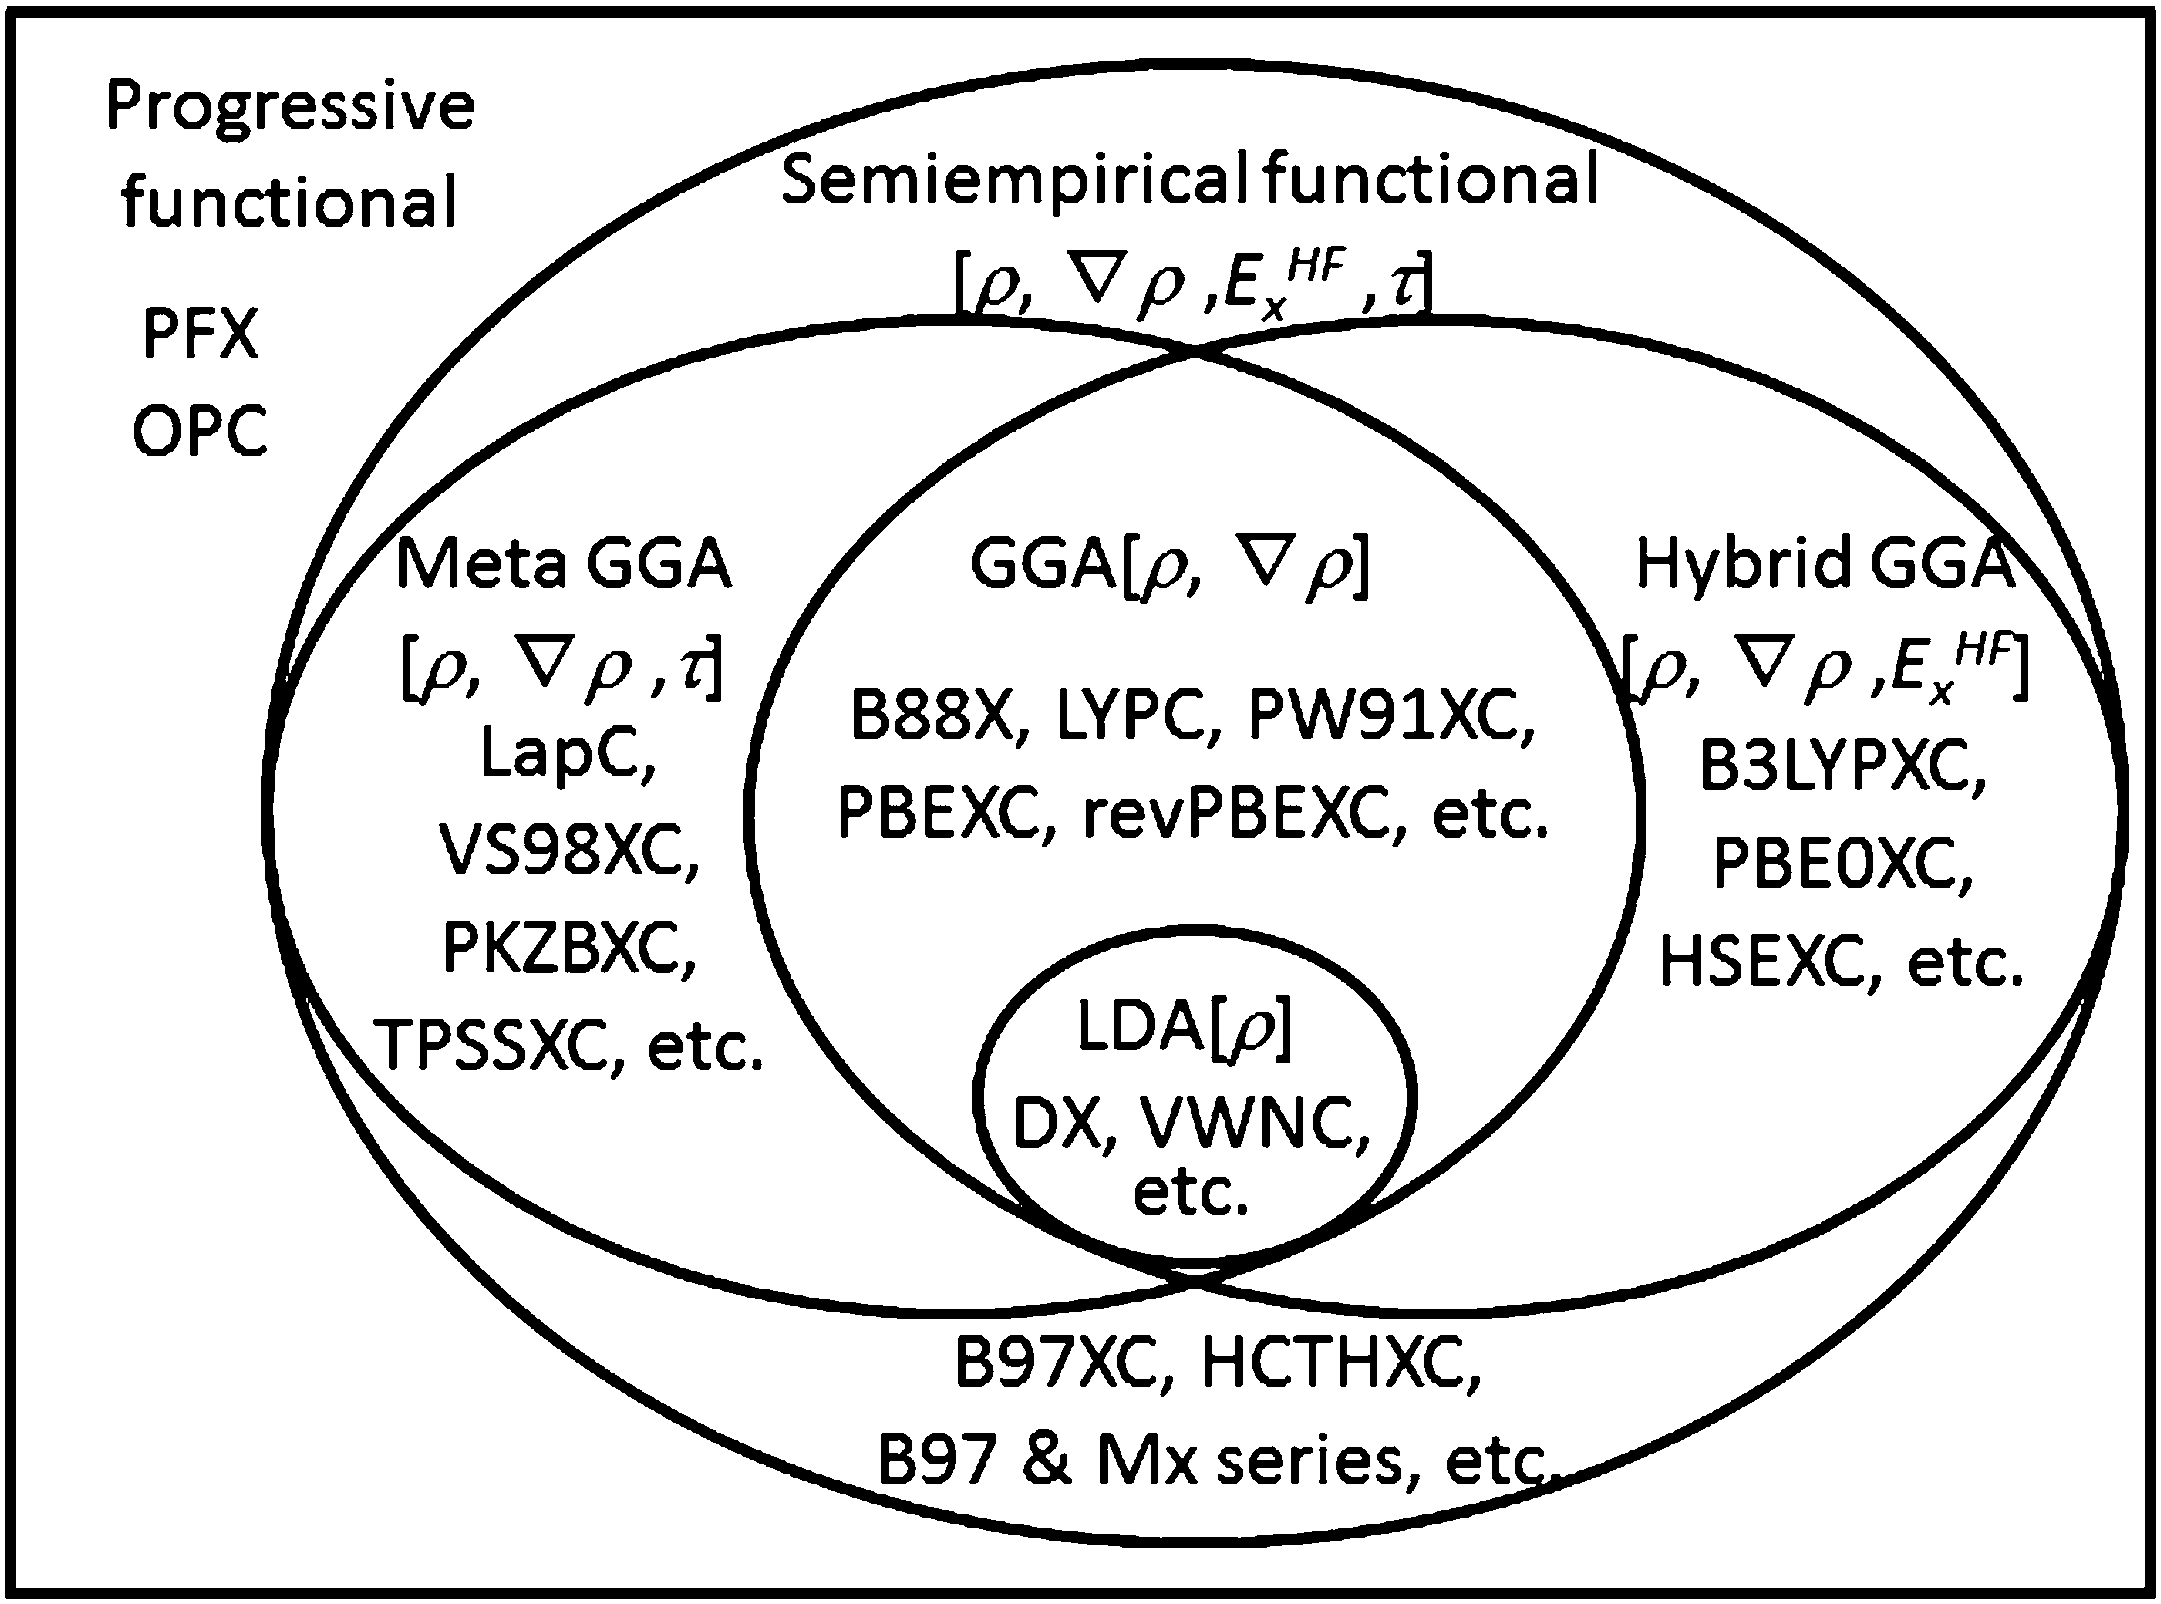
\includegraphics[width=0.5\textwidth]{functional-classification.png}
    \caption{交换-关联泛函的分类}
    \label{fig:excahnge-correlation-functional}
\end{figure}

目前并没有能够准确计算一切体系的$E_\text{XC}$,没有也是很正常的,因为很明显,这个泛函需要的复杂程度和“看着库仑相互作用想出一切可能的凝聚态现象”是一样的,后者眼下不可能做到,前者当然不可能做到。
但是对特定的体系,一些相互作用通道可以忽略,一些误差可以互相抵消,找到一个复杂程度适中的泛函描述它们是可以做到的。
适当地构造和选择泛函非常需要技术含量和经验。

最后,虽然原则上一切库仑相互作用导致的物理效应都可以通过$E_\text{XC}[\rho(\vb*{r})]$得到,这件事实际上做起来并不那么容易。
如果一个泛函被证明能够模拟一些相互作用通道导致的物理而无法模拟另一些,我们就需要手动向一个没有可调参数的$E_\text{XC}[\rho(\vb*{r})]$引入一些修正项。
这些修正项的大小往往无法固定下来,因为不同情况下$E_\text{XC}[\rho(\vb*{r})]$对对应的相互作用通道的忽略可能也是不一样的。
请注意交换关联泛函是通过计算\emph{电子数密度}具有某种特点的系统获得的,而不是通过分析哪些费曼图要保留哪些可以忽略获得的,一个泛函\emph{不能}良好地对应到一种通常意义上的保留一些相互作用而忽略另一些的有效模型上,交换关联泛函到底把什么纳入了考虑是缺乏直观的物理意义的,这也是DFT难以系统地提升精度的原因;在使用更加接近微扰场论方法的那些算法(如各种post-HF方法)时我们是清楚地知道自己忽略了什么的,在DFT中我们并不知道自己忽略了什么。
手动引入Hubbard排斥(所谓LDA+$U$,涉及非常短程的相互作用,不容易被比较光滑的泛函模拟)、范德瓦尔斯力(长程,不容易被比较局域的泛函模拟)就是例子。

\subsection{LDA近似}

本节考虑自旋不重要的系统,即无需考虑自旋-轨道耦合,无磁序等等的系统。
当电子密度变化非常平缓时,$\grad{\rho},\laplacian{\rho}$等全部可以看成是零,此时交换关联泛函的形式是
\begin{equation}
    E_\text{XC}[\rho(\vb*{r})] = \int \dd[3]{\vb*{r}} \rho(\vb*{r}) \epsilon_\text{XC}(\rho(\vb*{r})).
\end{equation}
这就是所谓的\concept{局域密度近似(LDA)}:每单位的交换关联能只和该地点的电子密度有关。
注意$\epsilon_\text{XC}$和$V_\text{XC}$不是一回事,两者的关系是
\begin{equation}
    V_\text{XC}(\vb*{r}) = \epsilon_{\text{XC}}(\rho(\vb*{r})) + \rho(\vb*{r}) \dv{\epsilon_\text{XC}}{\rho}.
\end{equation}

我们主要将尝试寻找一个确定适用于均匀电子气的交换关联泛函。均匀电子气指的是没有晶格、也没有外场时的库伦相互作用电子气,其电荷密度是处处均匀的。
对充分大的盒子中的均匀电子气,$E$正比于系统体积,从而$E / V$可以认为只依赖于电子数密度,和$V$没有直接的依赖关系。
对这样的体系,显然我们有
\begin{equation}
    \frac{N}{V} \epsilon_\text{XC}(N / V) \times V = E_\text{XC}.
\end{equation}
由于无论是均匀电子气还是电子密度较平缓但是的确有晶格周期势的电子气理论上均共享一种LDA近似适用的$E_\text{XC}$,而$\epsilon_\text{XC}(\rho(\vb*{r}))$只能看到$\vb*{r}$点的电子数密度,而不能够分辨电子数密度是否存在空间起伏,我们确定,$\epsilon_\text{XC}$可以按照如下方式得到:
\begin{equation}
    \epsilon_\text{XC}(\rho(\vb*{r})) = \eval{\left( \frac{E_\text{XC, homogeneous}}{N} \right)}_{N / V \to \rho(\vb*{r})}.
    \label{eq:from-homogeneous-electron-gas}
\end{equation}
换句话说,我们只需要计算具有不同电子数密度的均匀电子气的基态能量,按照上式即可拟合出$\epsilon(\rho(\vb*{r}))$的一个表达式。
因此LDA近似实际上是非常唯一的,不同的LDA泛函的区别仅仅在于拟合函数的形式不同。

在计算不同电子数密度的均匀电子气的基态能量时常常使用一种更加方便的记号。我们定义平均每个电子占据的球状体积的半径(所谓\concept{Wigner–Seitz半径})
\begin{equation}
    \frac{4\pi}{3} r_\text{s}^3 = \frac{1}{\rho},
\end{equation}
它和电子数密度一一对应。通常拟合$E$和$r_\text{s}$之间的关系,而不是$E$和$\rho$之间的关系。

\subsubsection{Hartree-Fock近似和托马斯-费米-狄拉克泛函}

自由电子气的基态就是费米面以内的每个轨道都占据了一上一下两个电子的状态,我们设共有$N$个电子,那么这些电子占据了$N/2$个不同的轨道。设这些轨道为$\{\phi_i(\vb*{r})\}$。
仅考虑库伦相互作用引入的一阶微扰,则有
\[
    E = \sum_{\sigma, \sigma'} \mel{\Psi}{
        \frac{1}{2} \int \dd[3]{\vb*{r}} \dd[3]{\vb*{r}'} {\psi}^\dagger_{\sigma}(\vb*{r}) {\psi}^\dagger_{\sigma'}(\vb*{r}') \frac{e^2}{\abs{\vb*{r} - \vb*{r}'}} {\psi}_{\sigma'}(\vb*{r}') {\psi}_\sigma(\vb*{r})
    }{\Psi}.
\]
这里必须完整地考虑自旋自由度的作用。可以使用Wick定理把上式展开,这就是在做Hartree-Fock近似。
请注意由于均匀电子气中没有自旋翻转,任何形如
\[
    \mel{\Psi}{{\psi}_\sigma^\dagger {\psi}_{\sigma'}}{\Psi}, \quad \sigma \neq \sigma'
\]
的项都是零,而
\[
    \mel{\Psi}{{\psi}^\dagger_\sigma(\vb*{r}) {\psi}_{\sigma}(\vb*{r}')}{\Psi} = \sum_i \phi_i^*(\vb*{r}) \phi_i(\vb*{r}'),
\]
于是最后能量修正为
\[
    E = \frac{1}{2} \int \dd[3]{\vb*{r}} \dd[3]{\vb*{r}'} \frac{e^2}{\abs{\vb*{r} - \vb*{r}'}} \bigg(
        \underbrace{4 \sum_{i} \abs{\phi_i(\vb*{r})}^2 \sum_{i} \abs{\phi_i(\vb*{r}')}^2}_\text{classical coulomb energy, Hartree term} - \underbrace{2 \sum_i \phi_i^*(\vb*{r}) \phi_i(\vb*{r}') \sum_i \phi_i^*(\vb*{r}') \phi_i(\vb*{r})}_\text{exchange energy}
    \bigg).
\]
交换能项前面的因子是$2$而不是$4$是因为自旋不同的电子之间的交换能全部抵消了。这样交换能或者说Fock项就是
\begin{equation}
    E_\text{X} = - \int \dd[3]{\vb*{r}} \dd[3]{\vb*{r}'} \frac{e^2}{\abs{\vb*{r} - \vb*{r}'}} \abs{\sum_i \phi_i^*(\vb*{r}) \phi_i(\vb*{r}')}^2 . 
    \label{eq:exchange-energy-homogeneous-gas}
\end{equation}
对箱归一化的均匀电子气,有
\[
    \phi_i(\vb*{r}) = \frac{1}{\sqrt{V}} \ee^{- \ii \vb*{k}_i \cdot \vb*{r}},
\]
于是就有
\begin{equation}
    \sum_i \phi_i^*(\vb*{r}) \phi_i(\vb*{r}') = \sum_{\text{occupied $\vb*{k}$}} \frac{1}{V} \ee^{\ii \vb*{k} \cdot (\vb*{r} - \vb*{r}')} = \frac{1}{(2\pi)^3} \int_{\abs{\vb*{k}} < k_\text{F}} \dd[3]{\vb*{k}} \ee^{\ii \vb*{k} \cdot (\vb*{r} - \vb*{r}')},
    \label{eq:homogeneous-density}
\end{equation}
而电子密度的一半(因为只考虑了轨道自由度)为
\[
    n(\vb*{r}) / 2 = \frac{k_\text{F}^3}{6 \pi^2}.
\]
于是我们通过$k_\text{F}$引入了电子数密度。
将\eqref{eq:homogeneous-density}代入\eqref{eq:exchange-energy-homogeneous-gas}就得到交换能的形式。
由于我们做了LDA近似,就是将每一个体积元看成一个箱子,这个箱子里面是均匀电子气,而忽略箱子和箱子之间的衔接,只有$\vb*{r} - \vb*{r}'$不超出一个箱子时\eqref{eq:homogeneous-density}才有明显的非零值。
每个箱子都有自己的费米动量,记作$k_\text{F}(\vb*{r})$(具体是关于$\vb*{r}$还是$\vb*{r}'$无关紧要因为两者总是在同一个箱子内;它们本质上都是$\rho(\vb*{r})$的函数)。
令
\[
    \vb*{s} = \vb*{r} - \vb*{r}', 
\]
则
\[
    \begin{aligned}
        E_\text{X} &= - e^2 \int \dd[3]{\vb*{r}} \dd[3]{\vb*{s}} \frac{1}{s} \abs{\frac{1}{(2\pi)^3} \int_{\abs{\vb*{k}} < k_\text{F}} \dd[3]{\vb*{k}} \ee^{\ii \vb*{k} \cdot \vb*{s}}}^2 \\
        &= - e^2 \int \dd[3]{\vb*{r}} \dd[3]{\vb*{s}} \frac{1}{s} \left( \frac{3}{2} \frac{\sin t - t \cos t}{t^3} \rho(\vb*{r}) \right)^2 \quad (t= k_\text{F}(\vb*{r}) s) \\
        &= - 9 e^2 \pi \int \dd[3]{\vb*{r}} \int \dd{t} \frac{t}{k_\text{F}(\vb*{r})^2} \rho(\vb*{r})^2 \left( \frac{\sin t - t \cos t}{t^3} \right)^2 \\
        &= - e^2 \frac{3}{4} \left( \frac{3}{\pi} \right)^{1/3} \int \dd[3]{\vb*{r}} \rho(\vb*{r})^{4/3}.
    \end{aligned}
\]
当然,根据\eqref{eq:from-homogeneous-electron-gas},可以不使用这种繁琐的方法,直接假定$\rho(\vb*{r})$是常数,计算完之后再将它换成$\rho(\vb*{r})$。总之,我们得到了\concept{托马斯-费米-狄拉克泛函}:
\begin{equation}
    E_\text{X}[\rho(\vb*{r})] / e^2 = - \frac{3}{4} \left( \frac{3}{\pi} \right)^{1/3} \int \dd[3]{\vb*{r}} \rho(\vb*{r})^{4/3} = - 0.7386 \int \dd[3]{\vb*{r}} \rho(\vb*{r})^{4/3}.
    \label{eq:thomas-fermi-dirac-functional}
\end{equation}
对均匀或不均匀但缓变的电子气这个泛函确定适用。
等价地说,我们有
\begin{equation}
    \epsilon_\text{X}(\rho(\vb*{r})) = - \frac{3}{4} \left(\frac{3}{\pi}\right)^{1/3} \rho(\vb*{r})^{1/3},
\end{equation}
或者使用$r_\text{s}$表示为
\begin{equation}
    \epsilon_\text{X} = % TODO
\end{equation}

对一般的系统,托马斯-费米-狄拉克泛函当然是不那么精确的,但是我们可以以它为更精确的泛函的起点。
\eqref{eq:thomas-fermi-dirac-functional}本质上是Hartree-Fock近似中的Fock项,那么要修正它,加入关联能就可以,即我们需要尝试寻找一个$E_\text{C}$使得
\begin{equation}
    E_\text{XC}[\rho(\vb*{r})] = E_\text{X}[\rho(\vb*{r})] + E_\text{C}[\rho(\vb*{r})].
\end{equation}
这个$E_\text{C}$就称为\concept{关联泛函}。

还应该提醒一点:实际上\eqref{eq:thomas-fermi-dirac-functional}甚至没有完整地考虑Fock项,因为它是在假定电子气是均匀的前提下计算出来的。
一般的自旋不重要的系统的Fock项,也就是\eqref{eq:hartree-fock-scf-spinless},是不能够写成电子数密度的泛函的,因为它依赖于多电子波函数的细节。
从这里也可以看出来密度泛函理论中交换关联泛函非物理的特点,因为物理量的解析表达式通常都是依赖于多电子波函数的细节的,将一切都使用电子数密度表示,实际上是不太容易做解析计算的。

\subsubsection{关联泛函的量子蒙特卡洛计算}

关联泛函就是正确的$E_\text{XC}$减去\eqref{eq:thomas-fermi-dirac-functional}。

通常使用量子蒙卡方法计算均匀电子气的基态能量,将它表示成$r_\text{s}$的函数做曲线拟合,就能够得到$\epsilon_\text{C}$。

常见的形式包括Perdew-Zunger,VWN等等。

\subsubsection{LDA近似的局限性}

普通的LDA泛函虽然将Hartree-Fock近似中的Fock项考虑了,但是由于要写出和$\rho(\vb*{r})$的显式依赖,LDA泛函给出的仅仅是均匀电子气的交换能,那么实际上会高估电子的离域特性而低估电子的定域特性。
如果我们要分析的系统中有电子比较定域,仅仅使用LDA泛函可能是不太可靠的。

LDA近似倾向于低估原子间距,理由也是显然的:如果电子比较离域,化学键可以比较强,从而原子被更加紧密地绑定在一起。

\subsection{LSDA近似}

现在转而考虑自旋系统的LDA近似。含自旋版本的托马斯-费米-狄拉克泛函需要将两种自旋分开计算,因为它们在\eqref{eq:hartree-fock-scf-with-spin}中就是分开的(不然也就不会导致等效的自旋-自旋相互作用了)。
回顾$E_\text{X}$的推导过程,我们先计算了轨道波函数的电子数密度,将它乘以2得到总的电子数密度,然后将\eqref{sec:hohenberg-kohn-theorem-spinless}中的Fock项(是用轨道波函数计算出Fock项以后乘以2得到的)表示成总的电子数密度的泛函。
对向上自旋重复以上步骤,则单独的向上自旋的电子贡献的交换能应该是$E_\text{X}[2 \rho_\uparrow(\vb*{r})] / 2$,因此含自旋的交换能是
\begin{equation}
    E_\text{X,spin}[\rho_\uparrow, \rho_\downarrow] = \frac{1}{2} (E_\text{X}[2 \rho_\uparrow(\vb*{r})] + E_\text{X}[2 \rho_\downarrow(\vb*{r})]).
\end{equation}

\subsection{GGA近似}

从LDA近似的推导中可以清楚地看到,一旦离开了均匀电子气模型,LDA近似的可靠性就不好说了。
对那些电子密度确定会有比较大的空间起伏的系统——比如说在我们需要精确计算分子结构时——LDA近似的精度不是特别好,此时有必要引入GGA近似。

\subsection{杂化泛函:将Hartree-Fock近似结合进DFT}

LDA近似和GGA近似都是所谓的“显式密度泛函”,即它们和电子数密度之间真的能够写下一个解析式。
但是我们也注意到,Kohn-Sham波函数$\phi_{n \vb*{k}}(\vb*{r} \sigma)$本身其实是电子数密度和$V_\text{ion}$的泛函,因此,如果$E_\text{XC}$依赖于Kohn-Sham波函数,其实是无伤大雅的:因为这这不过是说,$E_\text{XC}$同时依赖于$\rho(\vb*{r})$和$V_\text{ion}(\vb*{r})$,而我们知道$\rho(\vb*{r})$和$V_\text{ion}(\vb*{r})$包含了同样的信息。
因此其实我们可以不拘泥于写下显式的$E_\text{C}[\rho(\vb*{r})]$,完全可以让它依赖于Kohn-Sham波函数,这种做法\emph{仍然在}密度泛函理论的框架中。

允许交换关联泛函依赖于Kohn-Sham波函数有很大好处。既然眼下写出万能的泛函不太可能,我们往往需要针对不同的体系,从一族泛函中找出来一个。
手动地根据不同的系统选择不同的泛函是很常见的(如对电子数密度有很大空间起伏的系统最好不要用LDA),而允许交换关联泛函依赖于Kohn-Sham波函数,可能可以让泛函自动地适合我们要计算的系统。

例如,一个立刻可以注意到的结论就是,自洽Hartree-Fock近似实际上可以看成DFT的一种特例。我们称它对应的泛函为\concept{Hartree-Fock泛函},记作$E_\text{HF}$(这里不写出$\rho(\vb*{r})$,因为它和$\rho(\vb*{r})$的依赖关系是隐式的)。

对有非常局域的电子的系统,LDA甚至GGA泛函可能是不够准确的。% TODO
自洽Hartree-Fock近似可能能够给出更好的结果,虽然它完全忽略了电子关联。
一种很自然能够想到的办法是,不如将Hartree-Fock泛函和某些普通的泛函按照一定比例混合起来,可能能够兼顾关联能和电子的定域特性。
这就是\concept{杂化泛函}。

% TODO:对自相互作用的评估

\subsection{DFT+$U$}

\subsection{范德瓦尔斯力}

\section{Kohn-Sham方程的离散化和求解}

\autoref{alg:basic-kohn-sham}没有给出如下具体内容:如何引入凝聚态系统中原子核的位置、携带的电荷(从而确定材料中的电子总量)等信息,即如何适当地将$V_\text{ion}$和$\mu$引入以列写Kohn-Sham方程;\eqref{eq:kohn-sham-eq}本身是微分方程,它需要做适当的离散化才能被计算机求解,由于它是本征值问题,我们可以将$\phi_i(\vb*{r})$函数在适当的基底(量子化学中通常称为\concept{基组})下展开,这样只需要求解矩阵的本征值问题。

对一个一般的凝聚态系统,\eqref{eq:kohn-sham-eq}中涉及的单电子波函数的个数要比系统中电子的数目($10^{23}$量级)还要多,否则$\rho(\vb*{r})$的总量不可能正确。
介质中的电子数目是非常多的,从而直接求解\eqref{eq:kohn-sham-eq}并不现实。
然而晶体有周期性结构,这就大大简化了计算,因为只需要计算一个晶胞内的情况即可。
实际上,由于大部分情况下相互作用衰减得很快,我们完全可以假定液体等也有周期性边界条件,只不过此时的晶胞要取得非常大。
于是以下我们将DFT计算中被认为是周期性的单元称为\concept{超胞(supercell)},对固体通常要求超胞取最简单的形式,即原胞,对单分子、液体或是有杂质的系统等则需要取一个较大的超胞。
对杂质,超胞应该包括杂质周围足够大的体态。
对单分子,当超胞足够大时第一布里渊区足够小,从而计算出的所谓“能带”实际上和单独的一个个能级毫无区别。
我们需要指定超胞的几何形状,并且在超胞内给出各个原子核的位置。

凝聚态研究中,由于系统的离散平移对称性,\eqref{eq:kohn-sham-eq}此时也具有离散平移对称性,它的解——也就是$\phi_i(\vb*{r})$——可以看成某个以我们设定的超胞为原胞的晶体中的单电子波函数,从而Bloch定理\eqref{eq:bloch-wavefunction}成立,且$\phi_i(\vb*{r})$中的$i$应该替换成Bloch波矢$\vb*{k}$,能带编号$n$和自旋$\sigma$。(同样,到这里,所谓“能带编号”也未必对应着实际的系统中的能带电子的能带编号;如何诠释它还是不确定的)

在下面介绍的各种方法中可以看到,虽然DFT没有任何经验参数,并且将每一条可能的能带都纳入考虑,截断能、$\vb*{k}$点采样、赝势的选择、泛函的选择会显著影响计算精度,对它们的选择是需要一些经验的,虽然我们的确不需要根据实验数据拟合一些经验参数输入计算程序——或者,有时候,DFT模拟中其实也会出现经验参数。

\subsection{基于超胞和平面波的Kohn-Sham方程朴素求解方法}\label{sec:supercell-pwdft}

\subsubsection{平面波基组下的Kohn-Sham方程}

求解$\phi_{n \vb*{k}}(\vb*{r})$就是要求解$u_{n \vb*{k}}(\vb*{r})$。
由于\eqref{eq:bloch-wavefunction}中的$u(\vb*{r})$具有周期性,它可以被展开成用倒格矢标记的一系列傅里叶分量,因此我们有(为书写方便暂时略去自旋指标,即$\phi$和$c$都是二分量对象;需注意由于可能有自旋-轨道耦合,自旋\emph{不能}被认为是附加在能带指标上的标签)
\begin{equation}
    \phi_{n \vb*{k}}(\vb*{r}) = \frac{1}{\sqrt{V_\text{u.c.}}} \sum_{\vb*{G}} c_{n, \vb*{k}, \vb*{G}} \ee^{\ii (\vb*{k} + \vb*{G}) \cdot \vb*{r}},
\end{equation}
或者,考虑到$\vb*{k}$局限在第一布里渊区中而$\vb*{G}$是倒格矢,从$\vb*{k} + \vb*{G}$可以唯一确定$\vb*{k}$和$\vb*{G}$,有
\begin{equation}
    \phi_{n \vb*{k}}(\vb*{r}) = \frac{1}{\sqrt{V_\text{u.c.}}} \sum_{\vb*{G}} c_{n, \vb*{k} + \vb*{G}} \ee^{\ii (\vb*{k} + \vb*{G}) \cdot \vb*{r}}.
    \label{eq:dft-plane-wave}
\end{equation}
这种选取$\phi_i$的方法称为\concept{平面波DFT(PWDFT)}。
用平面波做基底的好处在于,首先,对自由电子气模型适用的体系它有直接的物理意义,其次,将波函数展开为平面波有成熟的快速傅里叶变换算法,这样效率很高。
这样做也有坏处,首先是只能处理晶格系统(否则需要不可数无限多个平面波),单分子必须放在一个比较大的晶格中才能够正确计算;其次,对高度局域的电子态以及原子核附近波函数的剧烈振荡,需要大量平面波,效率低下,这点可以部分通过赝势解决。

除了平面波以外还有很多常用的基底,比如高斯波包。
以高斯波包为基底是可以不需要任何赝势的,它能够更加精确高效地处理低轨道电子,从而相较于PWDFT能够更好地处理过渡金属等。

\eqref{eq:dft-plane-wave}中的$\vb*{G}$分量在\eqref{eq:kohn-sham-eq}的动能项部分为$(\vb*{k} + \vb*{G})^2 / 2m$,由于实际能够存储的傅里叶分量的个数是有限的,通常会引入一个\concept{截断能},对每个$\vb*{k}$,我们只保留对动能的贡献小于截断能的那些$\vb*{G}$。
这意味着我们忽略了空间尺度特别小的现象,并且忽略了一部分能量,但是如果对应的$c_{n, \vb*{k} + \vb*{G}}$不大就没有什么问题。

实际能够处理的晶体都是有限大小的,或者说实际的$\vb*{k}$的取值是第一布里渊区中离散的一些点。
这就是说,我们需要给出一种“第一布里渊区中的动量采样”。
显然,采样越密越好;可以使用$\vb*{k} \cdot \vb*{p}$来简化计算。

最后我们处理至今尚未提及的$V_\text{ion}$。
原则上可以将$V_\text{ion}$取成不同位置的原子的原子核的库伦势场的叠加,这相当于将材料中的所有电子都做了计算,即做了\concept{全电子计算},当然,这样在原子核附近会有非常剧烈的波函数变化,并且高度局域的内层电子都会出现,从而截断能必须取得非常高,基本上是不现实的。
一般来说用不到全电子计算,因为化学反应的能级不足以激发内层电子,而如\autoref{sec:pseudopotential}所述,外层电子感受到的势场可以用赝势取代:可以只计算外层电子,完全不计算内层电子,从而自始至终$V_\text{ion}$都是用赝势组合而成的,此时截断能可以设置得比较小,因为$\phi_{n \vb*{k}}(\vb*{r})$在靠近原子核的位置也不会发生剧烈振荡。
但这样就有一个问题:密度泛函理论需要\emph{全空间}的电子数密度,但是使用了赝势之后,原子核附近的电子数密度是不准确的。
如果需要使用赝势,Kohn-Sham方程中能够直接组合得到电子数密度的$\phi_i(\vb*{r})$实际上\emph{不是}计算中实际求解出的\emph{赝Kohn-Sham波函数},赝Kohn-Sham波函数服从的方程相比原本的Kohn-Sham方程是需要修改的。
本节采用最为朴素的办法,直接将$V_\text{ion}$当成库伦势处理,因此本节的朴素的算法其实是不现实的:纯平面波方法基本上都是赝势方法。

综上,朴素的PWDFT计算需要的输入信息有:
\begin{itemize}
    \item 晶体结构,这包括超胞以及各个原子在超胞内部的位置以及各个原子的类型;
    \item 各个原子的原子序数,用以确定核电荷;
    \item 第一布里渊区采样,即\eqref{eq:dft-plane-wave}中$\vb*{k}$的密集程度;
    \item 和材料的结构、原子、$\vb*{k}$点采样都无关的东西,如截断能、泛函选取等。
\end{itemize}

\subsubsection{不考虑自旋的朴素PWDFT算法}

\begin{algorithm}

    \DontPrintSemicolon
    \SetAlgoLined

    \KwData{初始电子密度$\rho_0(\vb*{r})$,交换关联泛函选取$E_\text{XC}[\rho(\vb*{r})]$,不同原子的原子序数$\{Z_i\}$,原胞结构,$\vb*{k}$点采样$K = \{\vb*{k}\}$,原胞中电子总数$N_\text{e}$,截断能$E_\text{cut}$,最大迭代次数$N_\text{max}$,所考虑的最大能带数目$n_\text{max}$,容差$\epsilon$}
    \KwResult{Kohn-Sham波函数$\phi_{n \vb*{k}}(\vb*{r})$和对应的本征值$\epsilon_{n \vb*{k}}$,迭代次数$i$}
    
    \For{$\vb*{k} \in K$}{
        根据$\frac{(\vb*{k} + \vb*{G})^2}{2m} < E_\text{cut}$确定需要考虑的$\vb*{G}$的取值范围$G$ \;
    } 

    $i = 1$ \;
    使用不同原子的原子序数和原胞结构构造$V_\text{ion}(\vb*{r})$,并按照\eqref{eq:momentum-space-potential-dft}做傅里叶变换 \;
    使用$\rho_0(\vb*{r})$计算$V_\text{H}$和$V_\text{XC}$,并按照\eqref{eq:momentum-space-potential-dft}做傅里叶变换 \;
    将$V_\text{ion}, V_\text{H}, V_\text{XC}$代入\eqref{eq:kohn-sham-eq-pw-minimal}求解,对每个$\vb*{k}$求前$n_\text{max}$个解,得到$\{c_{n, \vb*{k} + \vb*{G}}^{(1)}\}$和$\{\epsilon_{n, \vb*{k} + \vb*{G}}^{(1)}\}$ \;
    将$\{c_{n, \vb*{k} + \vb*{G}}^{(1)}\}$代入\eqref{eq:pw-minimal-expand}计算出$\{\phi_{n, \vb*{k} + \vb*{G}}^{(1)}\}$ \;
    将$\{\phi_{n, \vb*{k} + \vb*{G}}^{(1)}\}$代入\eqref{eq:kohn-sham-density-pw-minimal}计算得到$\rho_1(\vb*{r})$ \;
    \While{$\rho_i(\vb*{r})$和$\rho_{i-1}(\vb*{r})$的差别大于容差$\epsilon$且$i < N_\text{max}$}{
        使用$\rho_i(\vb*{r})$计算$V_\text{H}$和$V_\text{XC}$,并按照\eqref{eq:momentum-space-potential-dft}做傅里叶变换 \;
        将$V_\text{ion}, V_\text{H}, V_\text{XC}$代入\eqref{eq:kohn-sham-eq-pw-minimal}求解,对每个$\vb*{k}$求前$n_\text{max}$个解,得到$\{c_{n, \vb*{k} + \vb*{G}}^{(i+1)}\}$和$\{\epsilon_{n, \vb*{k} + \vb*{G}}^{(i+1)}\}$ \;
        将$\{c_{n, \vb*{k} + \vb*{G}}^{(i+1)}\}$代入\eqref{eq:pw-minimal-expand}计算出$\{\phi_{n, \vb*{k} + \vb*{G}}^{(i+1)}\}$ \;
        将$\{\phi_{n, \vb*{k} + \vb*{G}}^{(i+1)}\}$代入\eqref{eq:kohn-sham-density-pw-minimal}计算得到$\rho_{i+1}(\vb*{r})$ \;
        $i = i + 1$ \;
    }
    
    \Return{$i$,波函数$\{\phi^{(i)}_{n, \vb*{k} + \vb*{G}}\}$和本征值$\{\epsilon^{(i)}_{n, \vb*{k} + \vb*{G}}\}$}\;

    \caption{给定晶格和原子赝势,不考虑自旋的最朴素的PWDFT静态自洽计算}
    \label{alg:static-pwdft-minimal}
\end{algorithm}

我们现在可以给出完整的平面波计算的方程和步骤了。首先考虑一个没有必要考虑自旋极化的系统,此时只需要求解轨道部分即可。
以下我们给出一个最简单的PWDFT算法,不考虑$f$,则电子数密度为
\begin{equation}
    \rho(\vb*{r}) = 2 \sum_{n, \vb*{k} \text{ occupied}}  \phi_{n \vb*{k}}(\vb*{r}),
    \label{eq:kohn-sham-density-pw-minimal}
\end{equation}
而$\phi_{n \vb*{k}}$展开为
\begin{equation}
    \phi_{n \vb*{k}}(\vb*{r}) = \frac{1}{\sqrt{V_\text{u.c.}}} \sum_{(\vb*{k} + \vb*{G}) / 2m \leq E_\text{cut}} c_{n, \vb*{k} + \vb*{G}} \ee^{\ii (\vb*{k} + \vb*{G}) \cdot \vb*{r}},
    \label{eq:pw-minimal-expand}
\end{equation}
在此平面波基组下,Kohn-Sham方程是
\begin{equation}
    \begin{aligned}
        &\quad \sum_{( \vb*{k} + \vb*{G}') / 2m \leq E_\text{cut} } \left( \frac{(\vb*{k} + \vb*{G}') ^2}{2m} \delta_{\vb*{G} \vb*{G}'} + V_\text{ion}(\vb*{G} - \vb*{G}') + V_\text{H}(\vb*{G} - \vb*{G}') + V_\text{XC}(\vb*{G} - \vb*{G}') \right) c_{n, \vb*{k} + \vb*{G}'} \\
        &= \epsilon_{n, \vb*{k} + \vb*{G}} c_{n, \vb*{k} + \vb*{G}},
    \end{aligned}
    \label{eq:kohn-sham-eq-pw-minimal}
\end{equation}
其中动量空间的势能由
\begin{equation}
    V_\text{ion}(\vb*{r}) = \frac{1}{\sqrt{V_\text{u.c.}}} \sum_{\vb*{G}} V(\vb*{G}) \ee^{\ii \vb*{G} \cdot \vb*{r}}
    \label{eq:momentum-space-potential-dft}
\end{equation}
定义,$V_\text{H}(\vb*{G})$和$V_\text{XC}(\vb*{G})$类同。
将以上细节填充进\autoref{alg:basic-kohn-sham}中,我们得到\autoref{alg:static-pwdft-minimal},即所谓\concept{静态自洽计算}。(说是“静态”是因为有时候我们对晶体结构只有一个大概的猜测,此时需要做结构优化,即所谓\concept{结构优化自洽计算},这个是要变动晶体结构的,而静态自洽计算不变动晶体结构)
只要输入的晶体信息是准确的,交换关联泛函的质量足够好,我们就得到了外层电子的模拟结果。

\autoref{alg:static-pwdft-minimal}有不少可以扩充的地方。
在实际的DFT软件包中,通常不会将各次迭代的波函数和本征值留到计算结束再输出,而是在每次循环中把计算结果写入一个输出文件中,这样如果某一步计算失败了,已经写入的数据还可以用;也可以不以$\rho_0(\vb*{r})$为初始值而是以一组波函数为初始值。

\subsection{全电子计算的APW系列方法}\label{sec:dft-lapw}

\subsubsection{APW方法}

\begin{figure}
    \centering
    

\tikzset{every picture/.style={line width=0.75pt}} %set default line width to 0.75pt        

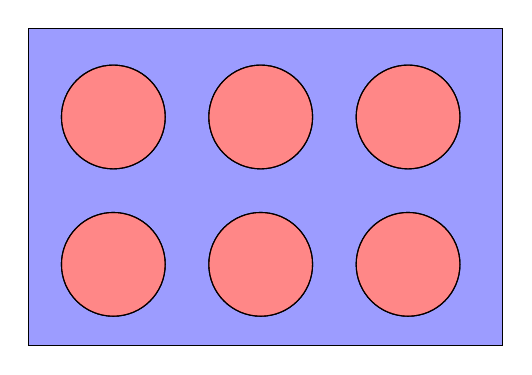
\begin{tikzpicture}[x=0.75pt,y=0.75pt,yscale=-1,xscale=1]
%uncomment if require: \path (0,300); %set diagram left start at 0, and has height of 300

%Shape: Rectangle [id:dp6984159445748599] 
\draw  [fill={rgb, 255:red, 0; green, 0; blue, 255 }  ,fill opacity=0.39 ] (215,60.24) -- (443.71,60.24) -- (443.71,213.24) -- (215,213.24) -- cycle ;
%Shape: Circle [id:dp8319615232565434] 
\draw  [fill={rgb, 255:red, 255; green, 255; blue, 255 }  ,fill opacity=1 ] (231,103) .. controls (231,89.19) and (242.19,78) .. (256,78) .. controls (269.81,78) and (281,89.19) .. (281,103) .. controls (281,116.81) and (269.81,128) .. (256,128) .. controls (242.19,128) and (231,116.81) .. (231,103) -- cycle ;
%Shape: Circle [id:dp09822489823753067] 
\draw  [fill={rgb, 255:red, 255; green, 255; blue, 255 }  ,fill opacity=1 ] (231,174) .. controls (231,160.19) and (242.19,149) .. (256,149) .. controls (269.81,149) and (281,160.19) .. (281,174) .. controls (281,187.81) and (269.81,199) .. (256,199) .. controls (242.19,199) and (231,187.81) .. (231,174) -- cycle ;
%Shape: Circle [id:dp3685610981270435] 
\draw  [fill={rgb, 255:red, 255; green, 255; blue, 255 }  ,fill opacity=1 ] (302,103) .. controls (302,89.19) and (313.19,78) .. (327,78) .. controls (340.81,78) and (352,89.19) .. (352,103) .. controls (352,116.81) and (340.81,128) .. (327,128) .. controls (313.19,128) and (302,116.81) .. (302,103) -- cycle ;
%Shape: Circle [id:dp09052649900670295] 
\draw  [fill={rgb, 255:red, 255; green, 255; blue, 255 }  ,fill opacity=1 ] (302,174) .. controls (302,160.19) and (313.19,149) .. (327,149) .. controls (340.81,149) and (352,160.19) .. (352,174) .. controls (352,187.81) and (340.81,199) .. (327,199) .. controls (313.19,199) and (302,187.81) .. (302,174) -- cycle ;
%Shape: Circle [id:dp9867069376310575] 
\draw  [fill={rgb, 255:red, 255; green, 255; blue, 255 }  ,fill opacity=1 ] (373,103) .. controls (373,89.19) and (384.19,78) .. (398,78) .. controls (411.81,78) and (423,89.19) .. (423,103) .. controls (423,116.81) and (411.81,128) .. (398,128) .. controls (384.19,128) and (373,116.81) .. (373,103) -- cycle ;
%Shape: Circle [id:dp07990038383333209] 
\draw  [fill={rgb, 255:red, 255; green, 255; blue, 255 }  ,fill opacity=1 ] (373,174) .. controls (373,160.19) and (384.19,149) .. (398,149) .. controls (411.81,149) and (423,160.19) .. (423,174) .. controls (423,187.81) and (411.81,199) .. (398,199) .. controls (384.19,199) and (373,187.81) .. (373,174) -- cycle ;

%Shape: Circle [id:dp3129249328243078] 
\draw  [fill={rgb, 255:red, 255; green, 0; blue, 0 }  ,fill opacity=0.47 ] (231,103) .. controls (231,89.19) and (242.19,78) .. (256,78) .. controls (269.81,78) and (281,89.19) .. (281,103) .. controls (281,116.81) and (269.81,128) .. (256,128) .. controls (242.19,128) and (231,116.81) .. (231,103) -- cycle ;
%Shape: Circle [id:dp596014249337059] 
\draw  [fill={rgb, 255:red, 255; green, 0; blue, 0 }  ,fill opacity=0.47 ] (231,174) .. controls (231,160.19) and (242.19,149) .. (256,149) .. controls (269.81,149) and (281,160.19) .. (281,174) .. controls (281,187.81) and (269.81,199) .. (256,199) .. controls (242.19,199) and (231,187.81) .. (231,174) -- cycle ;
%Shape: Circle [id:dp5835262974399322] 
\draw  [fill={rgb, 255:red, 255; green, 0; blue, 0 }  ,fill opacity=0.47 ] (302,103) .. controls (302,89.19) and (313.19,78) .. (327,78) .. controls (340.81,78) and (352,89.19) .. (352,103) .. controls (352,116.81) and (340.81,128) .. (327,128) .. controls (313.19,128) and (302,116.81) .. (302,103) -- cycle ;
%Shape: Circle [id:dp5179374857726964] 
\draw  [fill={rgb, 255:red, 255; green, 0; blue, 0 }  ,fill opacity=0.47 ] (302,174) .. controls (302,160.19) and (313.19,149) .. (327,149) .. controls (340.81,149) and (352,160.19) .. (352,174) .. controls (352,187.81) and (340.81,199) .. (327,199) .. controls (313.19,199) and (302,187.81) .. (302,174) -- cycle ;
%Shape: Circle [id:dp34026554549538424] 
\draw  [fill={rgb, 255:red, 255; green, 0; blue, 0 }  ,fill opacity=0.47 ] (373,103) .. controls (373,89.19) and (384.19,78) .. (398,78) .. controls (411.81,78) and (423,89.19) .. (423,103) .. controls (423,116.81) and (411.81,128) .. (398,128) .. controls (384.19,128) and (373,116.81) .. (373,103) -- cycle ;
%Shape: Circle [id:dp50099078742766] 
\draw  [fill={rgb, 255:red, 255; green, 0; blue, 0 }  ,fill opacity=0.47 ] (373,174) .. controls (373,160.19) and (384.19,149) .. (398,149) .. controls (411.81,149) and (423,160.19) .. (423,174) .. controls (423,187.81) and (411.81,199) .. (398,199) .. controls (384.19,199) and (373,187.81) .. (373,174) -- cycle ;






\end{tikzpicture}

    \caption{蛋糕模具基组,蓝色的区域为平面波,红色的区域为角部分为球谐函数、径向部分为贝塞尔函数的一系列函数的线性组合}
    \label{fig:muffin-tin}
\end{figure}

如前所述,使用平面波方法计算全电子问题有现实中难以克服的困难,即需要非常多的平面波来模拟原子核附近的电子行为。
那么一种很自然的想法就是,可以构造\concept{蛋糕模具基组}:如\autoref{fig:muffin-tin}所示,每个原子核附近的一个球形区域内(\concept{蛋糕模具区域}),基函数的值由各向同性的函数——某个径向函数乘以球谐函数,然后对$l, m$线性组合——给出,而除此以外的区域(\concept{间隙区域})中则为平面波。
这样的基组是所谓\concept{缀加平面波(augmented plane-wave, APW)}。
可以设
\begin{equation}
    \phi_{Elm}(\vb*{r}) = Y_{lm}(\vu*{r}) R_{El}(r),
\end{equation}
其中$E$是一个连续参数;需注意由于我们没有像求解真正的单原子问题一样,要求无穷远处波函数衰减得足够快,蛋糕模具区域内的Kohn-Sham波函数是需要不可数无穷多个基函数的。
通常可以这样产生$\phi_{Elm}(\vb*{r})$:指定一个球对称势场$V(r)$,设
\begin{equation}
    - \frac{1}{r^2} \dv{r} \left( r^2 \dv{R_{El}}{r} \right) + \left( \frac{l (l+1)}{r^2} + V(r) \right) R_{El}(r) = E R_{El}(r).
    \label{eq:apw-muffin-tin-inside}
\end{equation}
现在给定一个晶胞中各个原子的位置$\vb*{R}_\alpha$后,我们将Kohn-Sham波函数$\phi_{n \vb*{k}}(\vb*{r})$按照如下以$\vb*{G}$标记的基底展开:
\begin{equation}
    \phi_{\vb*{k} + \vb*{G}} = \begin{cases}
        \ee^{\ii (\vb*{k} + \vb*{G}) \cdot \vb*{r}}, \quad &\text{in the interstitial region}, \\
        \sum_{l, m} a_{lm} \phi_{Elm}(\vb*{r} - \vb*{R}_\alpha) , \quad &\text{in muffin-tin balls},
    \end{cases}
    \label{eq:apw-basis}
\end{equation}
其中$a_{lm}$指定为
\begin{equation}
    a_{lm} = 4 \pi \ee^{\ii \vb*{k} \cdot (\vb*{r} - \vb*{R}_\alpha)} \ii^l Y_{lm}^*(\vu*{k}) \mathrm{j}_{l}(k \abs*{\vb*{r} - \vb*{R}_\alpha}) / R_{El} (\abs*{\vb*{r} - \vb*{R}_\alpha}),
\end{equation}
这样可以满足蛋糕模具区域边界上波函数值连续的条件(导数则未必连续)。
然后我们发现,只要蛋糕模具球的半径不太大,能够保证球内本原子的库伦吸引势能占据主导地位,球内的$V_\text{eff}(\vb*{r})$的三个部分——晶格势能(此时就是单个原子的库伦势$Z e / r$)、Hartree项、交换关联等效势能——都可以认为是只依赖于$\abs*{\vb*{r} - \vb*{R}_\alpha}$,具有球对称性。
而如果我们选取\eqref{eq:apw-basis}中的$E$为$\epsilon_{n \vb*{k}}$,就能够保证各个蛋糕模具球中Kohn-Sham方程自动成立,只需要求解间隙区域内的Kohn-Sham方程即可。
因此我们就得到了一种自洽求解全电子Kohn-Sham方程的方法:首先从某个试探电子数密度出发计算$V_\text{XC}$,将结果和试探$E$代入\eqref{eq:apw-muffin-tin-inside}中,对不同的$\vb*{k}$计算得到$\{\phi_{\vb*{k}+\vb*{G}}\}_{\vb*{G}}$,然后据此基底求解Kohn-Sham方程,更新电子数密度和$E$。

APW方法的主要不足在于除了电子数密度以外,$E$也需要自洽求解,或者说Kohn-Sham方程在此框架下是非线性的($\phi_{\vb*{k} + \vb*{G}}$非线性地依赖于$E$)。
这个方法现在已经极少使用了,取而代之的是更加高效的LAPW方法。

\subsubsection{LAPW方法}

为了避免自洽求解$E$,我们不妨做一个$\phi_{Elm}(\vb*{r})$和$E$的关系的拟设。
我们选定一个参考能量$E_0$,在它附近计算$\phi_{\vb*{k}+G}$和$\pdv*{\phi_{\vb*{k}+\vb*{G}}}{E}$,以此计算$E$点的$\phi_{\vb*{k}+\vb*{G}}$的线性估计值(所谓的\concept{线性化缀加平面波(LAPW)}),然后用它展开$\phi_{n \vb*{k}}$并求解Kohn-Sham方程。
为了增加一点灵活性,我们不固定$\phi_{\vb*{k} + \vb*{G}}$和$E - E_0$之间的关系,并可以对每个$l$都选取一个不同的$E_0$(通常取为主要由轨道角动量为该$l$的轨道构成的能带的中间能量),设
\begin{equation}
    \phi_{\vb*{k} + \vb*{G}} = \begin{cases}
        \ee^{\ii (\vb*{k} + \vb*{G}) \cdot \vb*{r}}, \quad &\text{in the interstitial region}, \\
        \sum_{l, m} ( a_{lm} \phi_{E_0 lm}(\vb*{r} - \vb*{R}_\alpha) + b_{lm} \eval{\pdv{\phi_{Elm}}{E}}_{E=E_0, \vb*{r} - \vb*{R}_\alpha} ) , \quad &\text{in muffin-tin balls}.
    \end{cases}
\end{equation}
由于实际的Kohn-Sham波函数通常是比较光滑的,我们不妨用$\phi_{\vb*{k} + \vb*{G}}$在蛋糕模具球边界上的导数连续的条件确定$a_{lm}$和$b_{lm}$。
然后我们要求$E$总是$\epsilon_{n \vb*{k}}$,即可复用APW方法的求解过程。

\subsection{赝势方法}

全电子计算常常是不必要的,因此现在我们转而考虑怎么将赝势引入DFT计算。
做DFT计算实际上就是求解\eqref{eq:kohn-sham-eq-pw-minimal},这形式上仍然是一个单电子方程,因此总的来说,“计算单原子波函数,然后把外层电子高频振荡抹平而拟合出等效势”的做法仍然是适用的。
\autoref{sec:pseudopotential}中的做法不考虑任何电子-电子相互作用而计算内层电子的轨道,即把介质中的原子当成类氢原子,但是这样无疑精度非常糟糕。
我们要做的是在Kohn-Sham方程求解中适当地引入赝势。
主要的问题在于,由于密度泛函理论依赖全空间的电子数密度,使用赝势求解得到的赝波函数和$\rho(\vb*{r})$之间没有非常简单的\eqref{eq:kohn-sham-density}这样的关系,因为在原子核附近,用赝Kohn-Sham波函数根据\eqref{eq:kohn-sham-density}计算出来的电子数密度是不正确的,这也意味着赝Kohn-Sham波函数服从的方程中的$V_\text{XC}$不是简单的$\fdv*{E_\text{XC}}{\rho}$。
因此,除了构造柔和的势能以外,我们还需要找到一种从赝Kohn-Sham波函数获得正确的电子数密度的方法。
不同种类的赝势的从赝Kohn-Sham波函数获得正确的电子数密度的方法当然也是不一样的,或者说,不同种类的赝势对应的赝Kohn-Sham方程中$V_\text{XC}$的形式是不一样的。

我们做\concept{核心电子冻结近似},即认为晶体中其它原子的存在不会改变内层电子的行为(特别的,不会改变原子核附近的电子数密度),从而,使用单原子计算结果拟合出来的赝势在晶体中仍然是适用的。
我们实际上也隐含地假定Kohn-Sham方程求解出来的本征值较低的Kohn-Sham波函数对应着内层电子;这件事倒是没有什么争议,因为这些本征值较低的Kohn-Sham波函数贡献的电子数密度确实集中在原子核附近,它们肯定对应着内层电子的电子数密度,而由核心电子冻结近似,把它们丢弃是没有问题的,因为反正内层电子的电子数密度不怎么变化。

设我们对单原子已经求解出了如下的Kohn-Sham方程:
\begin{equation}
    - \frac{\laplacian}{2m} \phi_{nlm}(\vb*{r}) - \frac{Z e^2}{r} \phi_{nlm}(\vb*{r}) + V_\text{XC}[\rho(\vb*{r})] \phi_{nlm}(\vb*{r}) = \epsilon_{n} \phi_{nlm}(\vb*{r}), \quad \rho(\vb*{r}) = 2 \sum_{n, l, m} \abs*{\phi_{nlm}(\vb*{r})}^2.
\end{equation}
这里的$n, l, m$和原子物理中惯用的记号完全一致,由于系统具有旋转不变性,$\rho(\vb*{r})$也具有旋转不变性,因此$V_\text{XC}$也具有,因此Kohn-Sham本征值只和主量子数$n$有关。
我们将电子分成内层电子和外层电子(或者说价电子),前者被认为固定不动的,可以计算出其数密度:
\begin{equation}
    \rho_\text{core}(\vb*{r}) = 2 \sum_{\text{core $n, l, m$}} \abs*{\phi_{nlm}(\vb*{r})}^2.
\end{equation}
完整的数密度就是用价电子Kohn-Sham波函数计算出来的数密度加上$\rho_\text{core}(\vb*{r})$。
进一步,将$r_\text{C}$内的$\phi_{nlm}(\vb*{r})$“抹平”,得到$\tilde{\phi}_{nlm}(\vb*{r})$,然后根据$\phi_{nlm}(\vb*{r})$和$\tilde{\phi}_{nlm}(\vb*{r})$找到一种能够将赝Kohn-Sham波函数映射到原Kohn-Sham波函数并由此得到全空间的电子数密度的方法,并根据
\begin{equation}
    - \frac{\laplacian}{2m} \tilde{\phi}_{nlm}(\vb*{r}) + V_\text{PP} \tilde{\phi}_{nlm}(\vb*{r}) + V_\text{XC}[\rho(\vb*{r})] \tilde{\phi}_{nlm}(\vb*{r}) = \epsilon_{n} \tilde{\phi}_{nlm}(\vb*{r}), \quad \rho(\vb*{r}) = \rho_\text{core}(\vb*{r}) + \rho_\text{v}[\{\tilde{\phi}_{i}(\vb*{r})\}]
\end{equation}
计算出赝势$V_\text{PP}$(注意它可能不是局域的)。
于是,求解晶体中的Kohn-Sham方程
\begin{equation}
    \begin{aligned}
        &- \frac{\laplacian}{2m} \phi_{n \vb*{k}}(\vb*{r}) + V_\text{ion}(\vb*{r}) \phi_{n \vb*{k}}(\vb*{r}) + V_\text{XC}[\rho(\vb*{r})] \phi_{n \vb*{k}}(\vb*{r}) = \epsilon_{n \vb*{k}} \phi_{n \vb*{k}}, \\
        &\rho(\vb*{r}) = 2 \sum_{\text{occupied $n, \vb*{k}$}} \abs*{\phi_{n \vb*{k}}(\vb*{r})}^2
    \end{aligned}
\end{equation}
就转化为求解
\begin{equation}
    \begin{aligned}
        &- \frac{\laplacian}{2m} \tilde{\phi}_{n \vb*{k}}(\vb*{r}) + V_\text{PP}(\vb*{r}) \tilde{\phi}_{n \vb*{k}}(\vb*{r}) + \fdv{V_\text{XC}[\rho(\vb*{r})]}{\rho(\vb*{r})} \fdv{\rho_\text{v}}{\tilde{\phi}^*_{n \vb*{k}}(\vb*{r})} = \epsilon_{n \vb*{k}} \tilde{\phi}_{n \vb*{k}}, \\
        &\rho(\vb*{r}) = \rho_\text{v}[\{\tilde{\phi}_{n \vb*{k}}\}] + \sum_{\vb*{i}, \alpha} \rho_\text{core}(\vb*{r} - \vb*{R}_{\vb*{i} \alpha}),
    \end{aligned}
\end{equation}
其中$\alpha$标记一个晶胞中不同的原子。
只要核心电子冻结近似成立,求解以上赝Kohn-Sham方程组就充分地考虑了内层电子对价电子的排斥作用、充分地考虑了内层电子对原子核的库伦势场的屏蔽,等等,求解得到的在$r_\text{C}$外的Kohn-Sham波函数和全电子计算一致,并且可以使用比较少的平面波。

\subsubsection{模守恒赝势}

\subsubsection{超软赝势}



\subsection{PAW方法}\label{sec:dft-paw}

赝势方法可以用很少的平面波非常快速地计算各种系统,但是无法做全电子计算,而且合理性存疑;LAPW等方法可以做全电子计算,但是非常慢,而且合理性同样存疑。
\concept{投影缀加波法(projector augmented wave method, PAW)}是一种能够同时兼顾两种需求的方法,超软赝势和LAPW方法都是它的特例。
实际上,PAW方法的推导是如此简单和清晰,以至于我们甚至可以反过来,用它作为对赝势方法和LAPW方法的辩护。

我们总是可以在赝Kohn-Sham波函数和真实的Kohn-Sham波函数(在PAW方法的语境下这称为全电子Kohn-Sham波函数,因为它和全电子计算算出来的是一样的;或者说,全电子波函数\emph{不是}多体波函数)之间建立一个线性映射,不妨写为
\begin{equation}
    \phi_{n \vb*{k}} = \mathcal{T} \tilde{\phi}_{n \vb*{k}}.
\end{equation}
如果我们要求赝波函数在蛋糕模具球以外和全电子波函数完全一致,$\mathcal{T}$算符就可以写作
\begin{equation}
    \mathcal{T} = 1 + \sum_{\alpha} \mathcal{T}_\alpha,
\end{equation}
其中$\mathcal{T}_\alpha$将$\alpha$号原子周围的蛋糕模具球中的赝波函数映射成全电子波函数。

设我们DFT求解孤立原子已经得到了Kohn-Sham波函数
\begin{equation}
    \phi_{nlm}(\vb*{r}) = R_{nl}(r) Y_{lm}(\vu*{r}),
\end{equation}
我们将它在蛋糕模具球以外截断。通过一定方法我们可以让$R_{nl}(r)$“柔化”,减少它的零点,这样能够得到
\begin{equation}
    \tilde{\phi}_{nlm}(\vb*{r}) = \tilde{R}_{nl}(r) Y_{lm}(\vu*{r}).
\end{equation}
由于$\tilde{\phi}_{nlm}$之间未必正交,我们需要求出一组投影波函数$\{d_{nlm}\}$,满足
\begin{equation}
    \braket*{p_{nlm}}{\tilde{\phi}_{n' l' m'}} = \delta_{n n'} \delta_{l l'} \delta_{m m'},
\end{equation}
则一种很好的选择是
\begin{equation}
    \mathcal{T}_\alpha = \sum_{n, l, m} (\ket*{\phi_{nlm}} - \ket*{\tilde{\phi}_{nlm}}) \bra{p_{nlm}} |_{\vb*{r} \to \vb*{r} - \vb*{R}_\alpha}.
\end{equation}
这就得到了$\mathcal{T}$。

我们现在指定了一种\emph{线性}的从赝Kohn-Sham波函数获得全电子Kohn-Sham波函数。
现在任何使用全电子Kohn-Sham波函数计算的形如$\mel{\phi}{A}{\phi'}$的式子可以全部改写成关于赝Kohn-Sham波函数的式子了——只需要将$\phi$换成$\tilde{\phi}$,将$A$换成$\mathcal{T}^\dagger A \mathcal{T}$即可。
特别的,电子数密度现在是
\begin{equation}
    \rho(\vb*{r}) = \sum_{n, \vb*{k}} f_{n \vb*{k}} \int \dd[3]{\vb*{r}} \abs*{\psi_{n \vb*{k}}(\vb*{r})}^2  % TODO
\end{equation}

可以看到PAW方法是\emph{能够}给出全电子计算精度的结果的。
如果没有任何电子被划为“冻结”的核心电子,那么PAW就是全电子计算;如果有一些电子被划为冻结的核心电子,那么PAW算出的价电子仍然是全电子精度的。
因此PAW方法已经可以被当成全电子方法了,但是它似乎也可以看成一种赝势方法。
一个PAW赝势需要包含蛋糕模具球里面的$\phi_{nlm}$和$\tilde{\phi}_{nlm}$,以及核心电子的Kohn-Sham波函数。

\begin{info}{VASP软件包}{vasp}
    VASP是维也纳大学维护的一个商业DFT包,基于PWDFT,支持的赝势类型包括模守恒赝势、超软赝势和PAW赝势。
    其输入文件有四个,正好对应四种输入:
    \begin{itemize}
        \item \texttt{POSCAR},给出一个平行六面体超胞的三个初基格矢,以及各个原子的类型、数目,用笛卡尔坐标系或是晶体坐标系给出的坐标。
        \item \texttt{POTCAR},赝势文件。
        \item \texttt{KPOINTS},$\vb*{k}$动量采样(注意不是$\vb*{G}$采样,$\vb*{G}$采样由根据\texttt{PSCAR}计算出来的倒格矢和\texttt{INCAR}中给定的截断能规定),需要指定第一布里渊区中被纳入考虑的$\vb*{k}$。VASP提供多种自动生成这些$\vb*{k}$点的方法。
        \item \texttt{INCAR},计算中的参数,截断能、泛函选择、最大计算步数、能带数目、容差、蛋糕模具球半径等。
    \end{itemize}
\end{info}

\section{物理量测量和后处理}

本节讨论Kohn-Sham方程求解完成后怎样从计算结果解读出我们需要的各个物理量,在第一性原理计算的语境下也可以称为“非自洽计算”,因为就是拿到了电荷密度,然后算各种东西,无需迭代求解Kohn-Sham方程。
这件事是没那么容易的,基本上和基态电子密度有解析形式关系的量就是基态能量,基态能量实际上就是能量泛函作用在基态电子密度$\rho(\vb*{r})$之后的结果。
除此以外的东西——比如第一激发态能量——和Kohn-Sham方程求解结果之间都没有特别平凡的关系。

% TODO:类似于确定每一条带上的电子磁矩如何,电荷密度等等

\subsection{单电子诠释和能带}\label{sec:single-electron-in-dft}

\subsubsection{Kohn-Sham方程的解的物理意义}

在待计算的系统确实适用单电子诠释时,我们将\eqref{eq:kohn-sham-eq}和\eqref{eq:dyson-wave-eq}对比,很容易看出两者的相似之处。
如果Hartree项加上$V_\text{XC}$构成对自能$\Sigma$的一个良好模拟,那么\eqref{eq:kohn-sham-eq}解出的$\epsilon_i$\emph{就是}经过相互作用修饰的能带电子的能量,或者说是费米液体中的$\epsilon_{\vb*{k}}$。
如果实际情况确实如此,那么\eqref{eq:dft-variation-principle}中的$\mu$实际上就是费米能,因为对比\eqref{eq:dft-variation-principle}和\eqref{eq:dft-variation-principle-shem}会发现
\begin{equation}
    \mu = \sum_{i=1}^N \epsilon_i.
\end{equation}

当然,如前所述,Kohn-Sham方程的推导的每一步都没有给出足够的条件让我们知道Kohn-Sham波函数到底是什么东西。
Kohn-Sham方程解得的本征值和本征函数到底是什么实际上是仍然有疑问的。
有一点是确定的,就是它们\emph{不严格是}单电子能量和波函数,因为已经证实,把它们当成单电子能量和波函数会产生系统的误差。
这其中最为著名的就是\emph{半导体能隙问题},即将DFT计算出来的Kohn-Sham本征值当作电子能量的话会倾向于系统地低估半导体的能隙,从而实验上明确确定是半导体的体系用DFT计算出来的能带结构看起来似乎是金属的。
关于这一误差到底在哪里没有特别明确的结论,因为DFT中不确定的、物理意义不清楚的东西非常多,首先我们不知道LDA和GGA这些非常局域的方法以及它们的推广是否足够精确,其次我们也不知道Kohn-Sham方程的解的物理意义是什么。

无论如何,Kohn-Sham方程的解至少提供了对单电子能量和波函数的一种估计,这意味着它可以作为物理意义清楚的场论方法的初始值。
如果真的如果需要非常可靠的能谱,总是可以以Kohn-Sham方程的解为初始值做诸如GW这样的进一步计算。

\subsubsection{GW计算}

GW计算实际上是一种独立的数值计算方法,但是因为它要求一个比较接近实际情况的单电子波函数作为起点,我们仍然可以将它视为DFT的后处理的一部分,即将DFT计算出来的Kohn-Sham波函数作为GW计算的初始值。
GW计算也是一种基于自能的计算方法,其中,它

\subsection{原子受力}



在计算单原子受力时我们最好把晶胞扩张得大一些。如果使用原胞做计算,那么将某个原子移动一小段得同时,其它原胞中与它地位一致的原子也发生了移动,因此通过这种方式计算原子移动前后的能量变化并进一步计算力是不准确的。
相反,如果晶胞被扩张了,那么移动一个原子之后,与之最为接近的那些原胞中与之地位一致的原子并没有发生移动,会给出相对可靠的结果。

\subsubsection{声子谱计算}

\section{结构优化和分子动力学模拟}

有时候我们对晶体结构只有一个大概的猜测,此时需要做结构优化,即所谓\concept{结构优化自洽计算}。

\concept{ab initio MD}

\section{DFT的推广版本}

\subsection{含时DFT(TDDDFT)}

Runge-Gross (RG) 定理的地位和Hohenberg-Kohn定理是一样的。